\documentclass[12pt,a4paper,oneside]{article}
\usepackage{lmodern}
\usepackage[T1]{fontenc}
\usepackage[polish]{babel}
\usepackage{polski}
\usepackage{indentfirst}
\usepackage{enumitem}
\usepackage{fancyhdr}
\usepackage{graphicx}
\usepackage{float}
\usepackage{hyperref}
\hypersetup{
    colorlinks,
    citecolor=black,
    filecolor=black,
    linkcolor=black,
    urlcolor=black
}
\setlist{nolistsep}
\pagestyle{fancy}
\selectlanguage{polish}
\setlength{\headheight}{15pt}

% % rozszerzenie nieco strony
% \setlength{\topmargin}{-1cm} \setlength{\textheight}{24.5cm}
% \setlength{\textwidth}{17cm} \addtolength{\hoffset}{-1.5cm}
% \setlength{\parindent}{0.5cm} \setlength{\footskip}{2cm}
\linespread{1.2} % odstęp pomiędzy wierszami

%%%% ŻYWA PAGINA %%%%%%%%%%%
\newcommand{\tl}[1]{\textbf{#1}}
\pagestyle{fancy}
\renewcommand{\sectionmark}[1]{\markright{\thesection\ #1}}
\fancyhf{} % usuwanie bieżących ustawień
\fancyhead[LE,RO]{\small\bfseries\thepage}
\fancyhead[LO]{\small\bfseries\rightmark}
\fancyhead[RE]{\small\bfseries\leftmark}
\renewcommand{\headrulewidth}{0.5pt}
\renewcommand{\footrulewidth}{0pt}
\addtolength{\headheight}{0.5pt} % pionowy odstęp na kreskę
\fancypagestyle{plain}{%
\fancyhead{} % usuń p. górne na stronach pozbawionych numeracji
\renewcommand{\headrulewidth}{0pt} % pozioma kreska
}

\begin{document}
{
\begin{titlepage}
    \fancyhf{}
    \headheight = 0pt
    \headsep =0pt
    \begin{center}
        \frenchspacing
        \thispagestyle{empty}
        \makeatletter
        \setlength\@fptop{0\p@ \@plus 1fil}
        \begin{figure}
            \centering
            
\includegraphics[width=0.4\textwidth,keepaspectratio]{images/politechnika_sl_logo_pion_pl_rgb.png}
        \end{figure}
        \makeatother
        {\large
            % Politechnika Śląska\\
            Wydział Informatyki, Elektroniki i Informatyki}

        \vfill
        \textbf{\Huge
            Aplikacja do zarządzania budżetem domowym}
        \vspace*{1\baselineskip}

        {\large \scshape
            Tworzenie Aplikacji Bazodanowych}
        \vfill

        {\small
            \begin{itemize}
                \item Mateusz Cudzik\\
                \item Jakub Ferens\\
                \item Mateusz Górecki\\
                \item Szymon Maciąg\\
                \item Kajetan Sommer\\
                \item Julia Wojciuch
            \end{itemize}
            \vspace*{1\baselineskip}
            % \vspace{0pt plus 0.5fill}

            Gliwice\\
            \today
        }
        \vspace*{0\baselineskip}
    \end{center}
\end{titlepage}
}

\thispagestyle{empty}
\tableofcontents
\newpage

\section{Wstęp}
Celem projektu jest stworzenie aplikacji do zarządzania domowym budżetem i jego
monitorowania. Warunkiem koniecznym jest obsługiwanie logowania, co umożliwi
korzystanie z niej wielu użytkownikom. Aplikacja pozwoli na tworzenie raportów
oraz kategoryzowanie przychodów i wydatków z różnych kont.

\section{Określenie wymagań}
\subsection{Wymagania funkcjonalne}
\begin{itemize}
    \item Obsługa logowania,
    \item Kategorie wydatków/przychodów,
    \item Kategorie kont,
    \item Transakcje między profilami,
    \item Generowanie raportów — analiza finansowa,
    \item Przechowywanie skanów paragonów/faktur,
    \item Przechowywanie dłużników,
    \item Informacje przechowywane w bazie danych,
    \item Dodawanie profilów członków rodziny do konta (profil dziecka, rodzica
          itd.),
    \item Dodanie konta bankowego i operacji na nim,
    \item Obsługa wydatków i przychodów.
\end{itemize}

\subsection{Wymagania niefunkcjonalne}
\begin{itemize}
    \item Bezpieczeństwo — okresowe tworzenie kopii zapasowych danych,
    \item Zabezpieczenie profili użytkowników hasłem,
    \item Hierarchia użytkowników — różne poziomy uprawnień/dostępu,
          ograniczenia dla profilów młodszych użytkowników,
    \item Użyteczność — aplikacja z przystępnym i łatwym w obsłudze interfejsem
          zarówno dla starszych, jak i młodszych użytkowników,
    \item Wieloplatformowość — przypadku aplikacji webowej dostępność z różnych
          urządzeń przy pomocy dowolnego systemu posiadającego przeglądarkę,
    \item System/Aplikacja przystosowana do łatwego rozwoju, rozbudowy i
          aktualizacji,
    \item Responsywność — odpowiedź aplikacji na działania użytkownika w
          określonym czasie (przykładowo do trzech sekund).
\end{itemize}

\section{Analiza MoSCoW}
\subsection{Must}
\begin{itemize}
    \item Przechowywanie informacji w bazie danych,
    \item dodawanie wydatków i przychodów,
    \item generowanie raportów,
    \item założenie konta i przypisania do niego danych,
    \item informowanie użytkownika o aktualnym stanie konta, który jest
          zmieniany wraz z kolejnymi wpisami o przychodach/wydatkach.
\end{itemize}

\subsection{Should}
\begin{itemize}
    \item Przypomnienie hasła,
    \item formularz rejestracji dostępny dla użytkownika,
    \item dzielenie wydatków i przychodów na kategorie,
    \item generowanie raportów z podziałem wydatków/przychodów na kategorie,
    \item operacje zarządzania profilami (dodawanie, usuwanie itd.).
\end{itemize}

\subsection{Could}
\begin{itemize}
    \item Potwierdzenie rejestracji mailem,
    \item edycja informacji o koncie (nazwy użytkownika, hasła itd.),
    \item ustawianie cyklicznych/stałych wydatków/przychodów,
    \item transakcje między profilami,
    \item przechowywanie skanów paragonów/faktur,
    \item definiowanie własnych, niestandardowych kategorii.
\end{itemize}

\subsection{Won't}
\begin{itemize}
    \item Weryfikacja Captcha,
    \item przechowywanie informacji o dłużnikach,
    \item powiadomienia o przekroczonym budżecie.
\end{itemize}

\section{Scenariusze przypadków użycia}
\subsection{Logowanie}
\subsubsection{Scenariusz główny logowania}
\begin{itemize}
    \item Przypadek rozpoczyna się, gdy niezalogowany użytkownik wejdzie
          na stronę.
    \item Użytkownik wpisuje swój login oraz hasło.
    \item System sprawdza poprawność danych.
    \item Użytkownik zostaje przeniesiony do panelu wyboru profilu.
    \item Użytkownik wybiera profil.
    \item Wyświetlony zostaje panel sterowania budżetem.
    \item Użytkownik zostaje zalogowany.
\end{itemize}

\subsubsection{Scenariusze poboczne logowania}
\paragraph{Konto nie istnieje}
\begin{itemize}
    \item Użytkownik zostaje przeniesiony do formularza rejestracji.
    \item Użytkownik wprowadza swoje dane.
    \item System sprawdza poprawność danych.
    \item Konto zostaje utworzone.
\end{itemize}

\paragraph{Wybrany profil jest chroniony}
\begin{itemize}
    \item Użytkownik wpisuje PIN.
    \item System sprawdza poprawność danych.
    \item W przypadku wprowadzenia poprawnego kodu pin scenariusz się kończy,
          w przeciwnym razie użytkownik jest informowany o błędnym kodzie PIN,
          po kilku błędnych próbach nakładana jest czasowa blokada.
\end{itemize}

\paragraph{Wybrany profil jest profilem dziecka}
\begin{itemize}
    \item Użytkownikowi wyświetlone zostaje uproszczone GUI.
\end{itemize}

\subsection{Dodawanie przychodów/wydatków}
\subsubsection{Scenariusz główny dodawania przychodów/wydatków}
\begin{itemize}
    \item Zalogowany użytkownik decyduje się dodać przychód/wydatek na panelu
          sterowania budżetem.
    \item Użytkownik wpisuje kwotę, nazwę własną operacji oraz wybiera jej
          kategorię.
    \item Operacja zostaje uwzględniona w budżecie.
\end{itemize}

\subsubsection{Scenariusze poboczne dodawania przychodów/wydatków}
\paragraph{Użytkownik dodaje własną kategorię}
\begin{itemize}
    \item Użytkownik podaje nazwę i wybiera kolor.
    \item Kategoria zostaje dodana do listy wszystkich kategorii.
\end{itemize}

\paragraph{Użytkownik dodaje wydatek przekraczający saldo}
\begin{itemize}
    \item Użytkownik zostaje ostrzeżony za pomocą powiadomienia przed wykonaniem
          operacji.
    \item Użytkownik anuluje lub potwierdza wykonanie transakcji.
\end{itemize}

\section{Diagram UML}
\begin{figure}[H]
    \rotatebox{90}{
        \begin{minipage}{\textheight}
            \thispagestyle{empty}
            \centering
            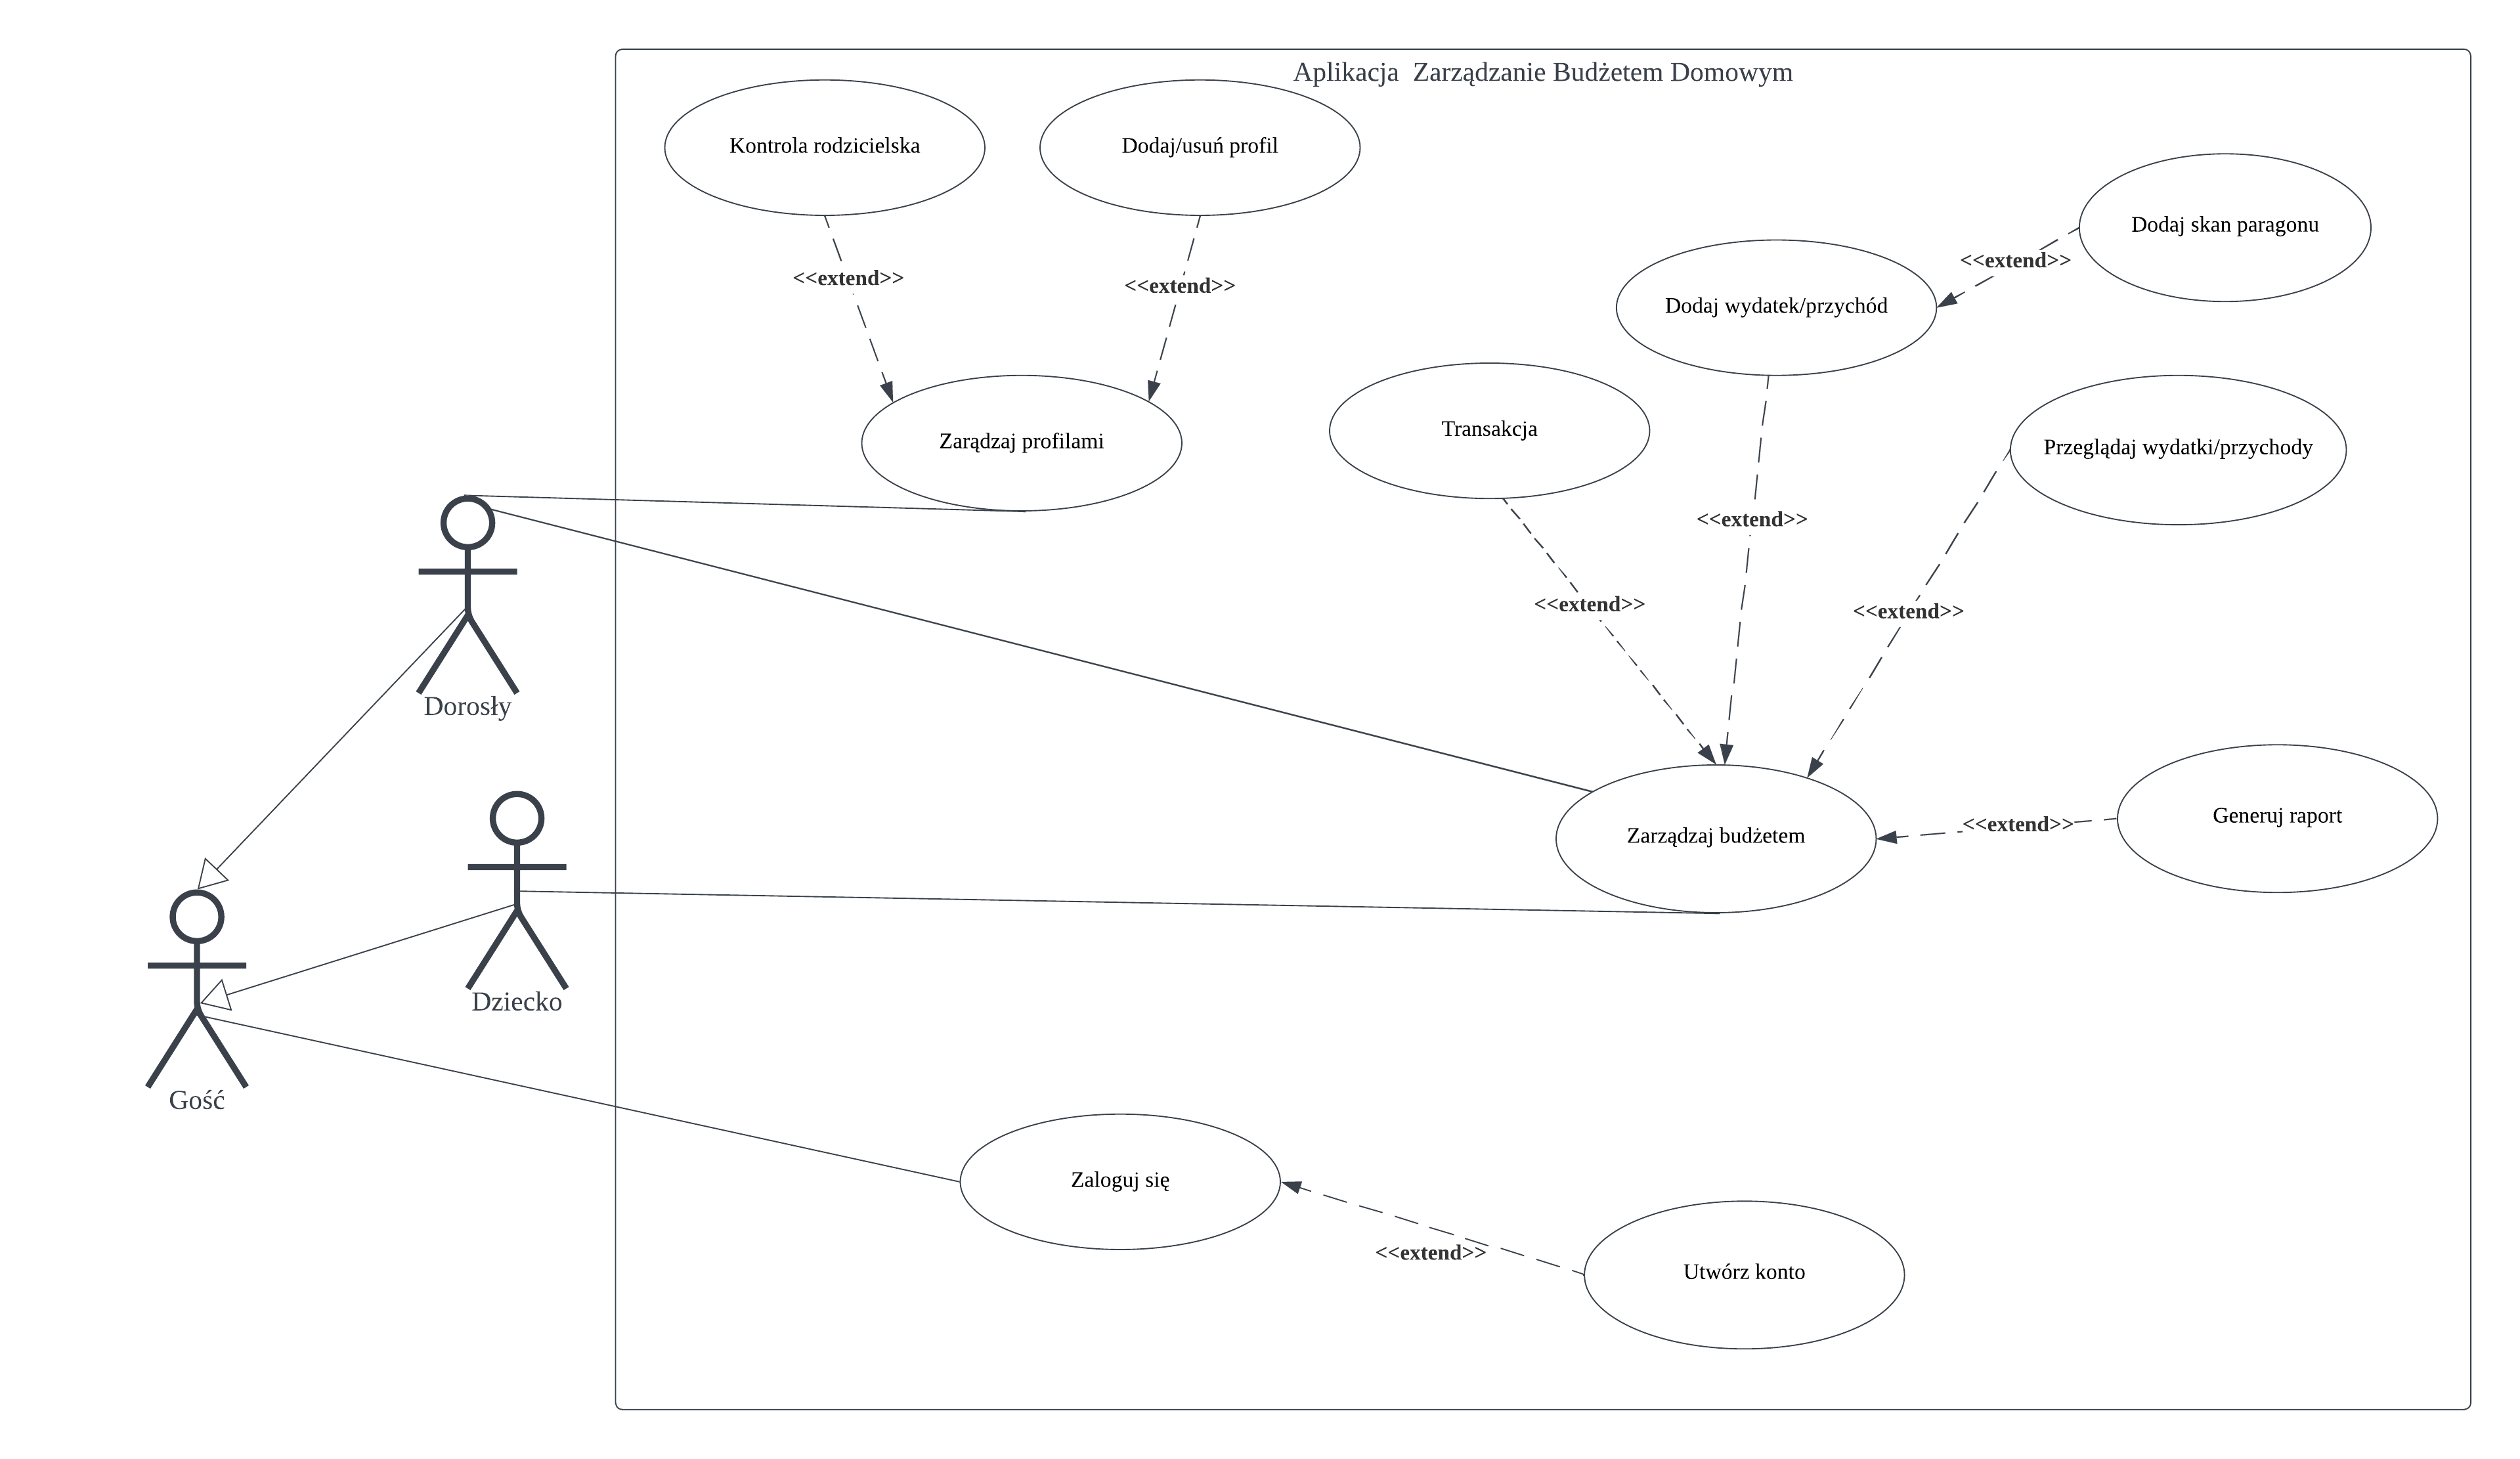
\includegraphics[width=\hsize,keepaspectratio]{images/UML1.png}
            \caption{Diagram UML.}
        \end{minipage}}
\end{figure}

\section{Schemat bazy danych}
\begin{figure}[H]
    \centering
    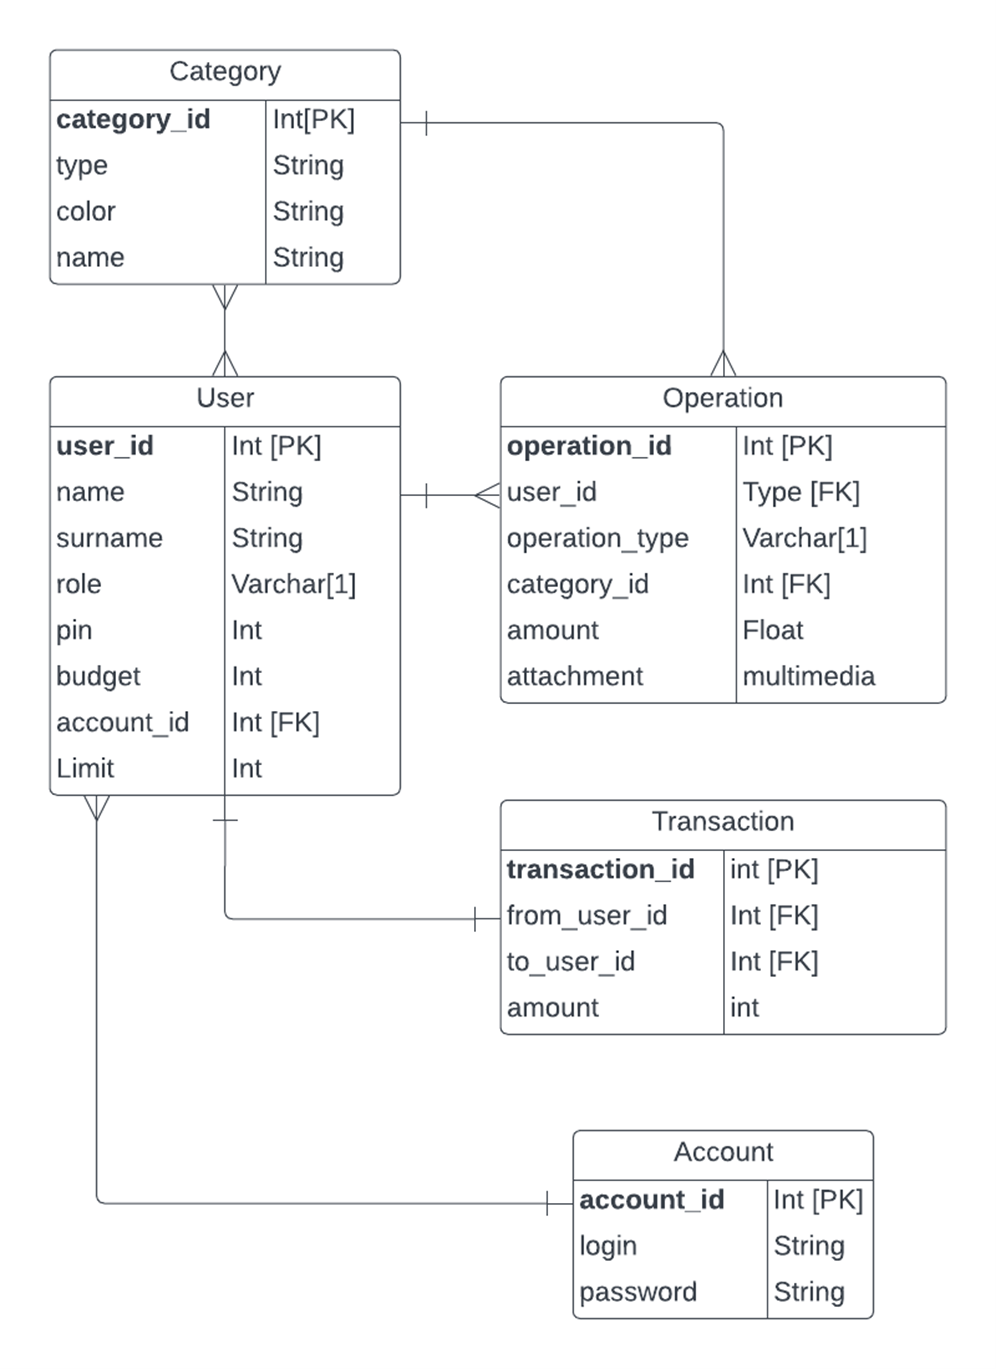
\includegraphics[width=\hsize,keepaspectratio]{images/DB1.png}
    \caption{Prototypowy schemat bazy danych}
\end{figure}

\section{Specyfikacja zewnętrzna}
\subsection{Rejestracja}
\subsubsection{Rejestracja konta użytkownika}
\begin{figure}[H]
    \centering
    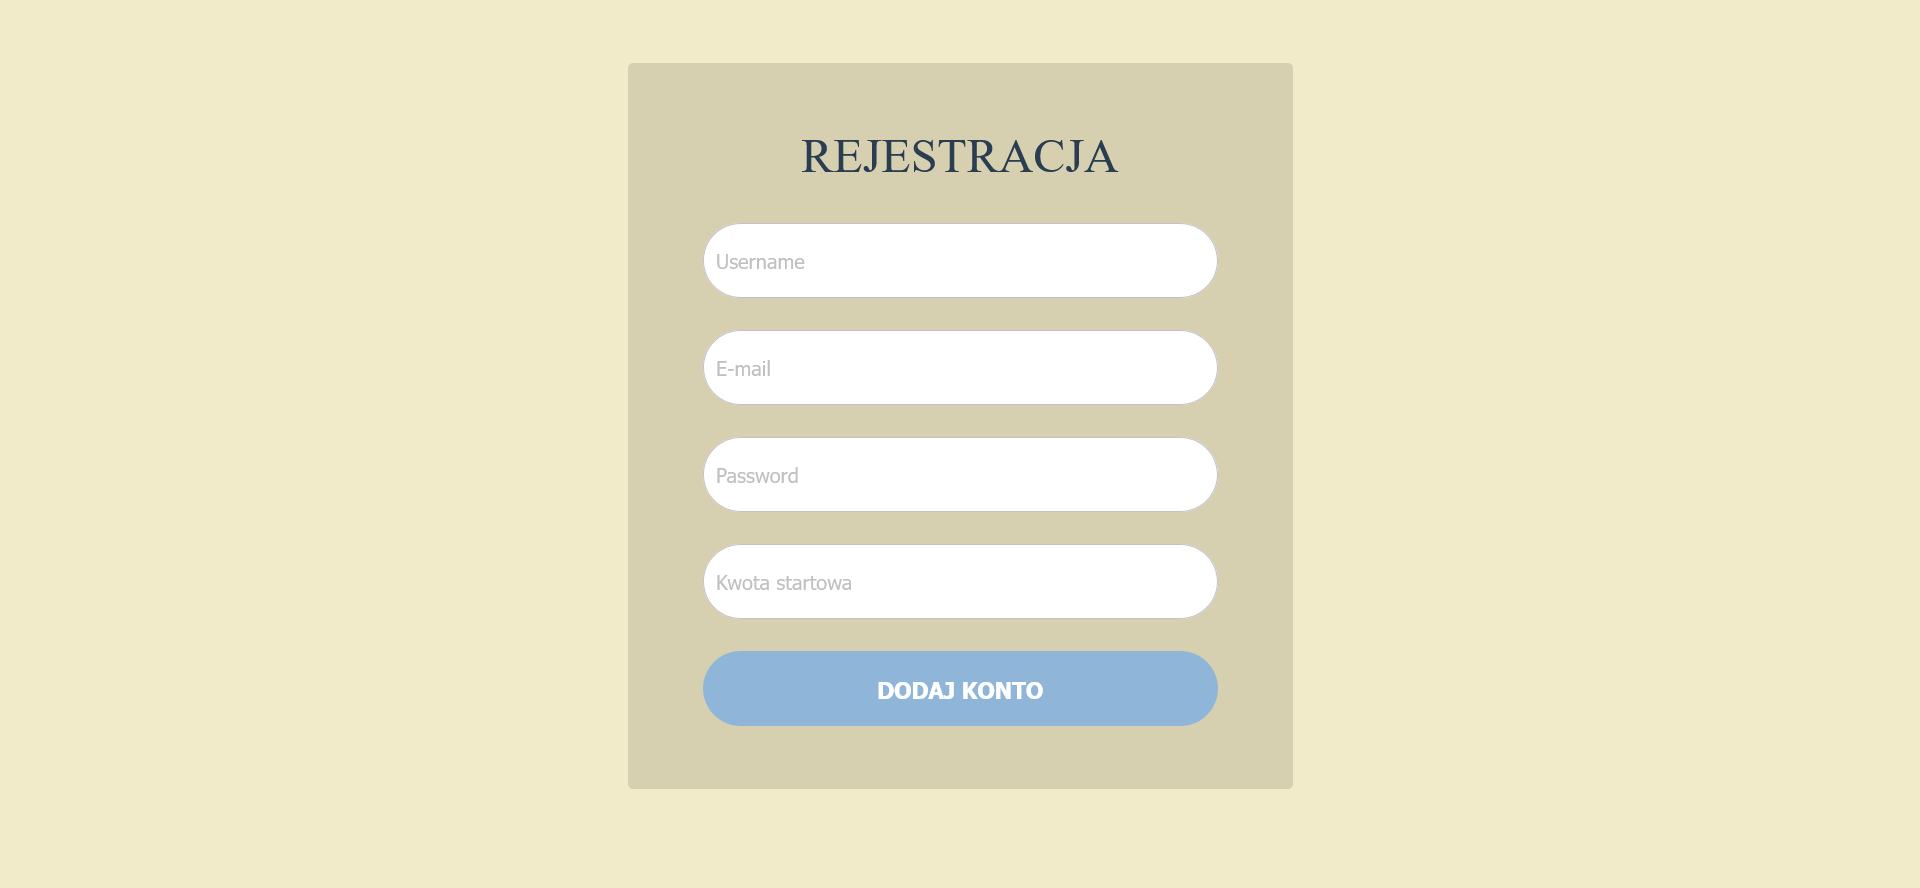
\includegraphics[width=\hsize,keepaspectratio]{images/register.png}
    \caption{Zrzut ekranu rejestracji}
\end{figure}
Użytkownik, chcąc skorzystać z aplikacji, musi posiadać własny profil. Formularz
rejestracyjny pozwala założyć konto. Celem założenia konta użytkownik musi podać:
\begin{itemize}
    \item nazwę użytkownika
    \item adres e-mail
    \item hasło
    \item kwotę początkową.
\end{itemize}
Naciśnięcie przycisku \textbf{DODAJ KONTO} skutkuje dodaniem konta do bazy danych.

\begin{figure}[H]
    \centering
    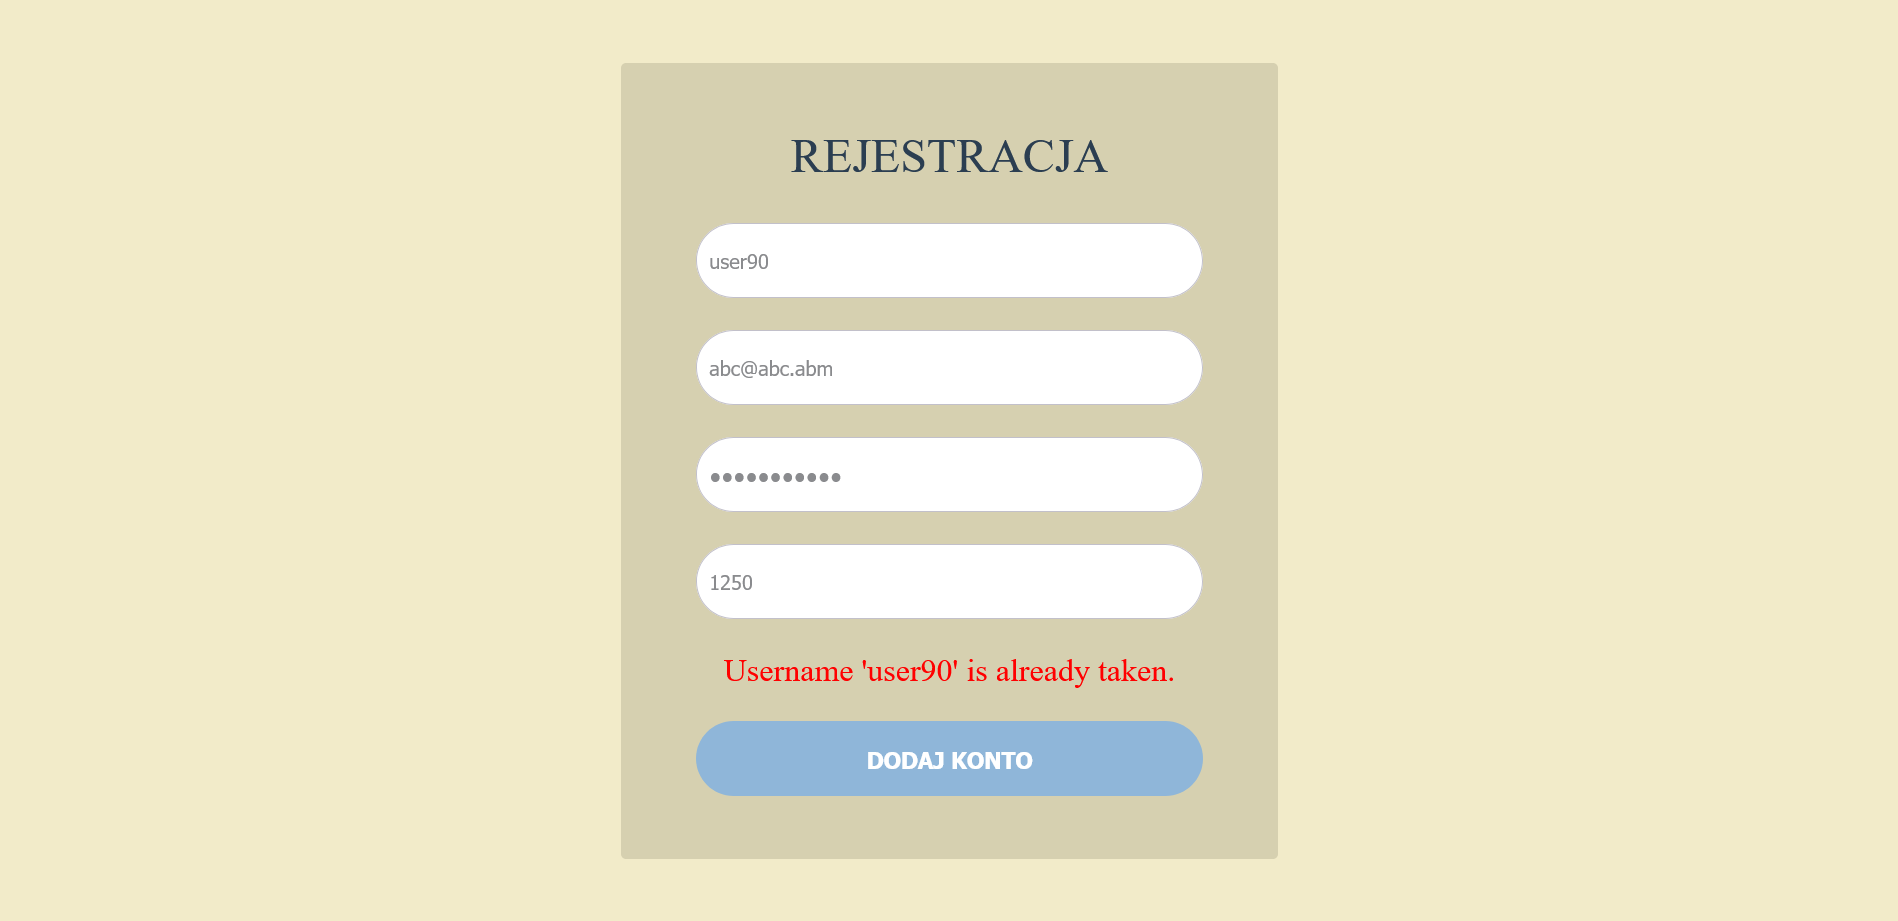
\includegraphics[width=\hsize,keepaspectratio]{images/register_account_exists.png}
    \caption{Zrzut ekranu rejestracji zakończonej niepowodzeniem.}
\end{figure}
Jeżeli w bazie danych istnieje konto o takich samych danych, system informuje
użytkownika o niemożności jego założenia stosownym komunikatem.

\subsubsection{Rejestracja konta dziecka}
\begin{figure}[H]
    \centering
    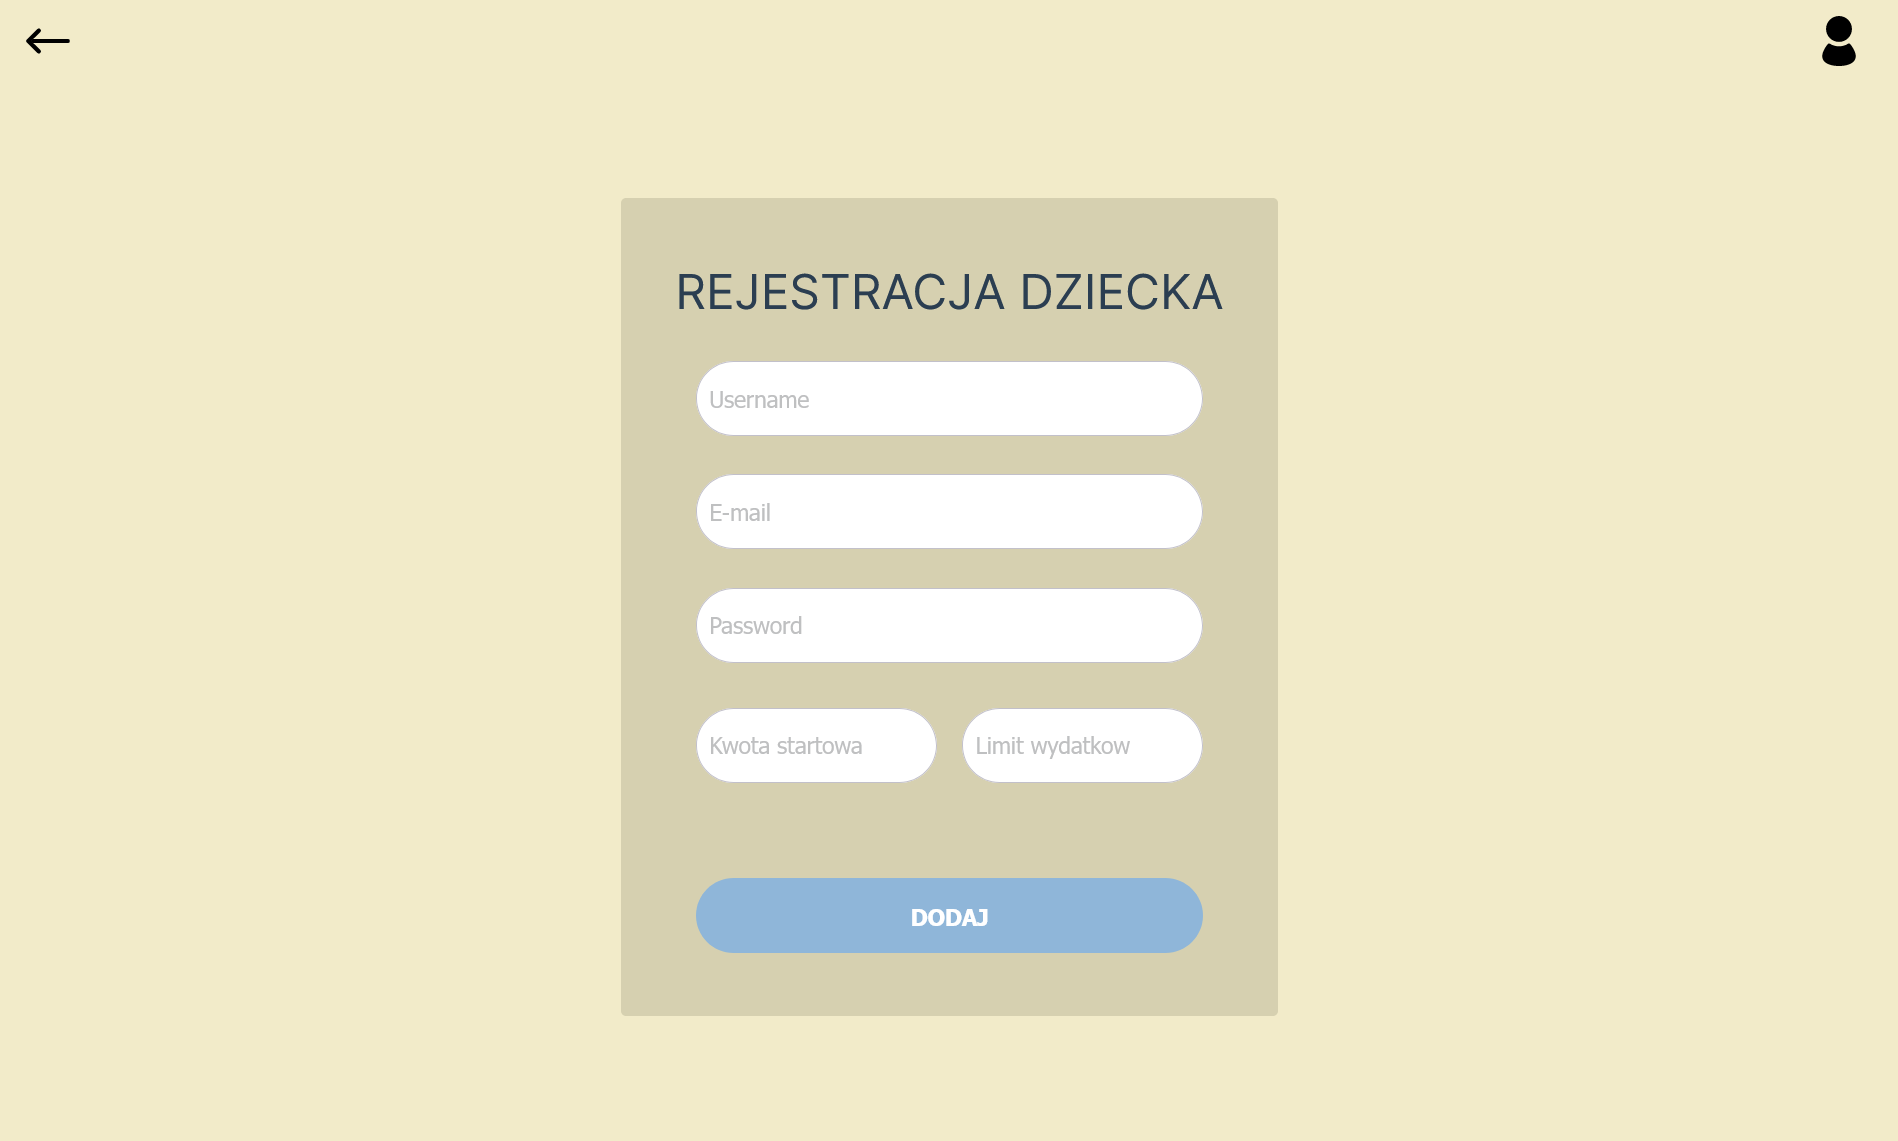
\includegraphics[width=\hsize,keepaspectratio]{images/register_childs_profile.png}
    \caption{Zrzut ekranu rejestracji konta dziecka.}
\end{figure}
Użytkownik dorosły może założyć konto o ograniczonym dostępie dedykowanie
dzieciom. Zasadniczą różnicą jest możliwość nadania limitu wydatków przypisanego
do tego typu profilu.

\subsection{Logowanie}
\begin{figure}[H]
    \centering
    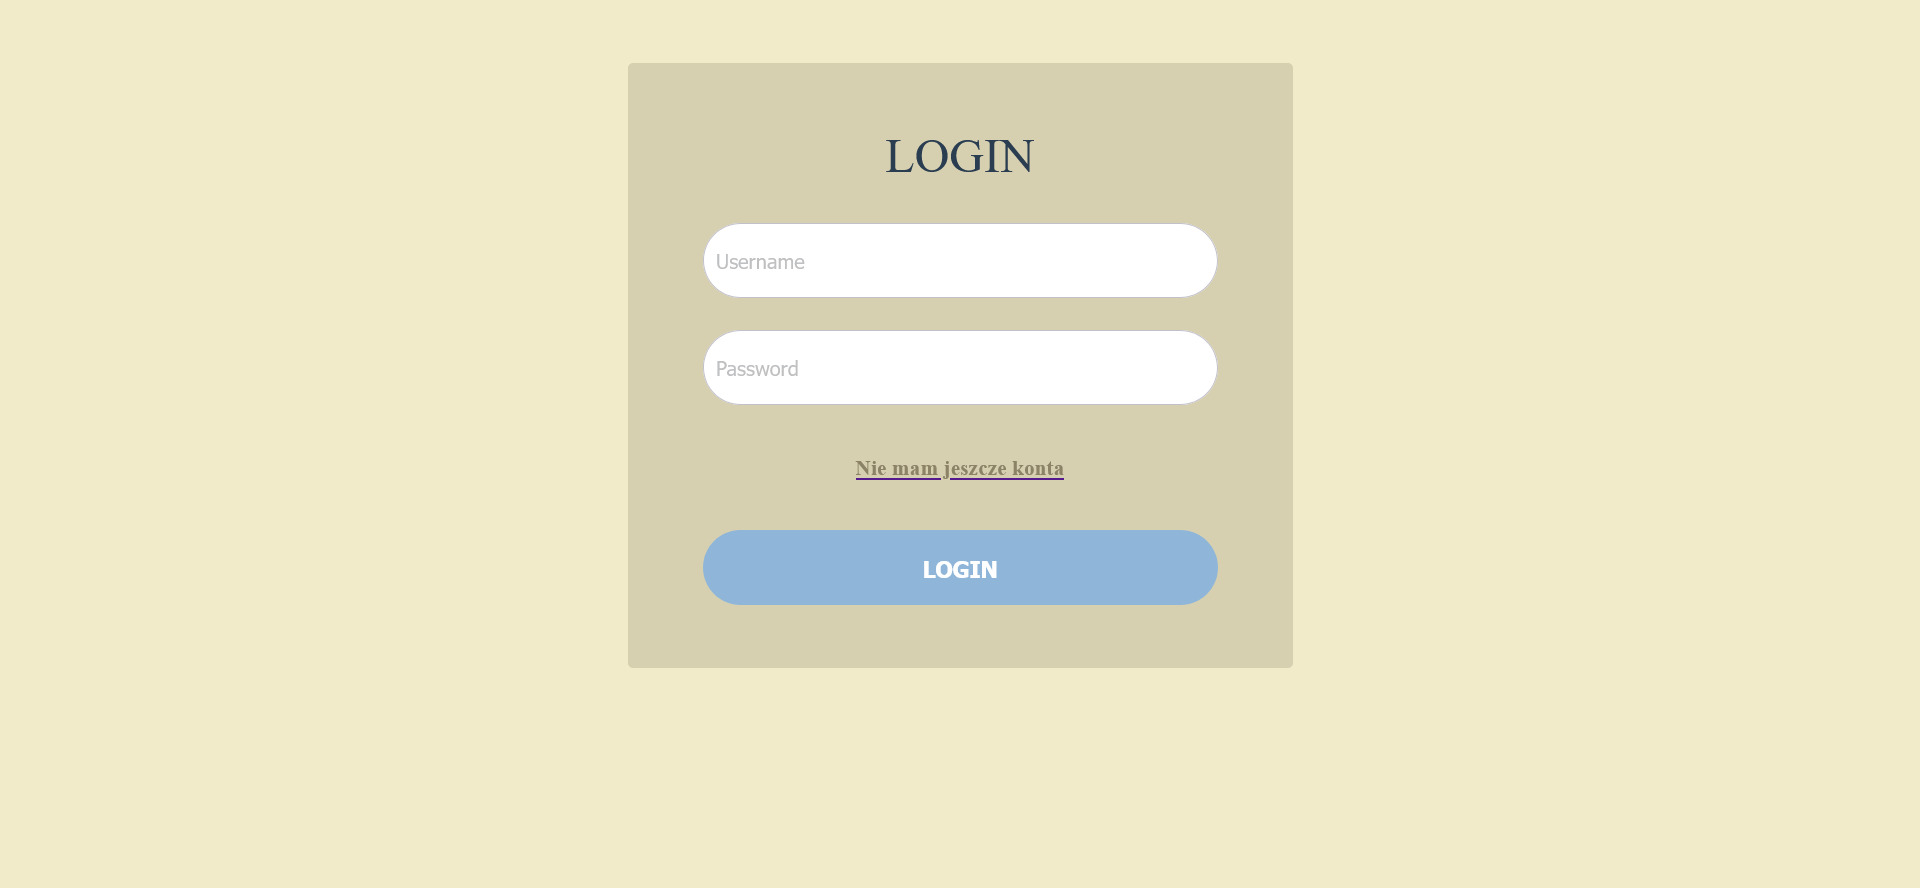
\includegraphics[width=\hsize,keepaspectratio]{images/login.png}
    \caption{Zrzut ekranu logowania.}
\end{figure}
Strona logowania zawiera formularz, w którym należy wprowadzić login użytkownika
oraz hasło. Po wprowadzeniu poprawnych danych oraz naciśnięciu przycisku
\textbf{LOGIN} użytkownik zostaje przeniesiony do ekranu głównego aplikacji.
Jeżeli użytkownik nie posiada konta, może w prosty sposób przejść do formularza
rejestracji, klikając w odnośnik \textbf{Nie mam jeszcze konta}.

\begin{figure}[H]
    \centering
    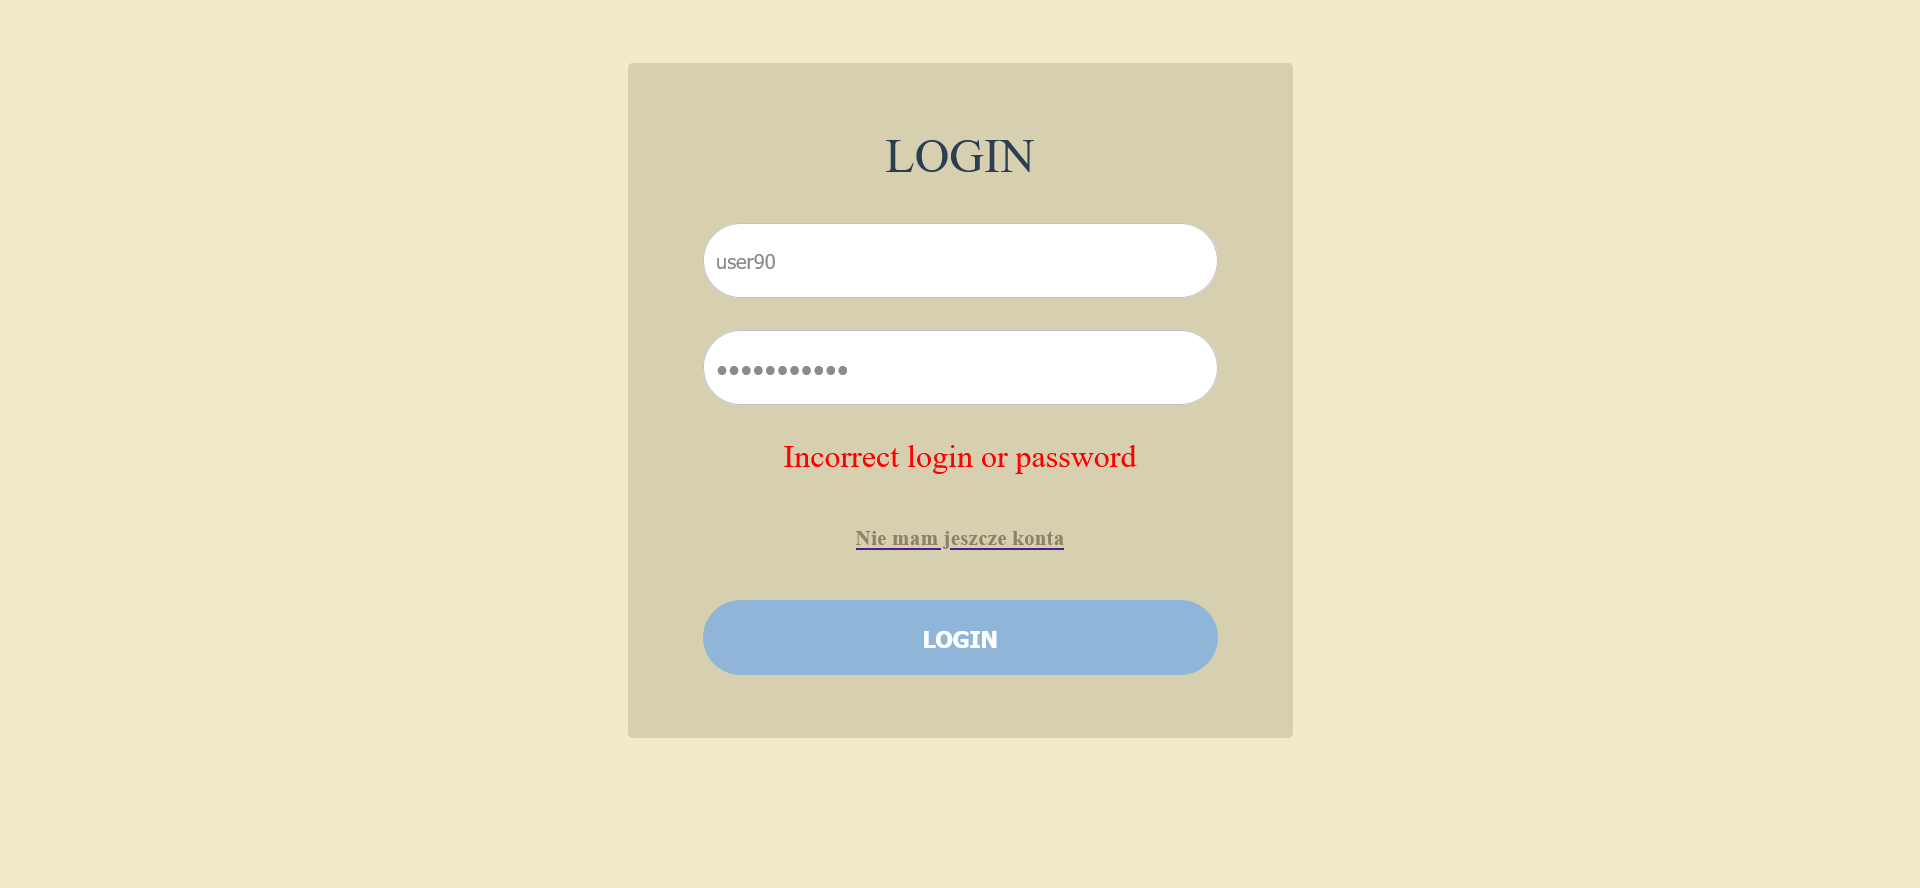
\includegraphics[width=\hsize,keepaspectratio]{images/login_failed.png}
    \caption{Zrzut ekranu błędnego logowania.}
\end{figure}
W przypadku podania niepoprawnych danych użytkownik jest informowany o fakcie
stosownym komunikatem.

\subsection{Ekran główny}
\begin{figure}[H]
    \centering
    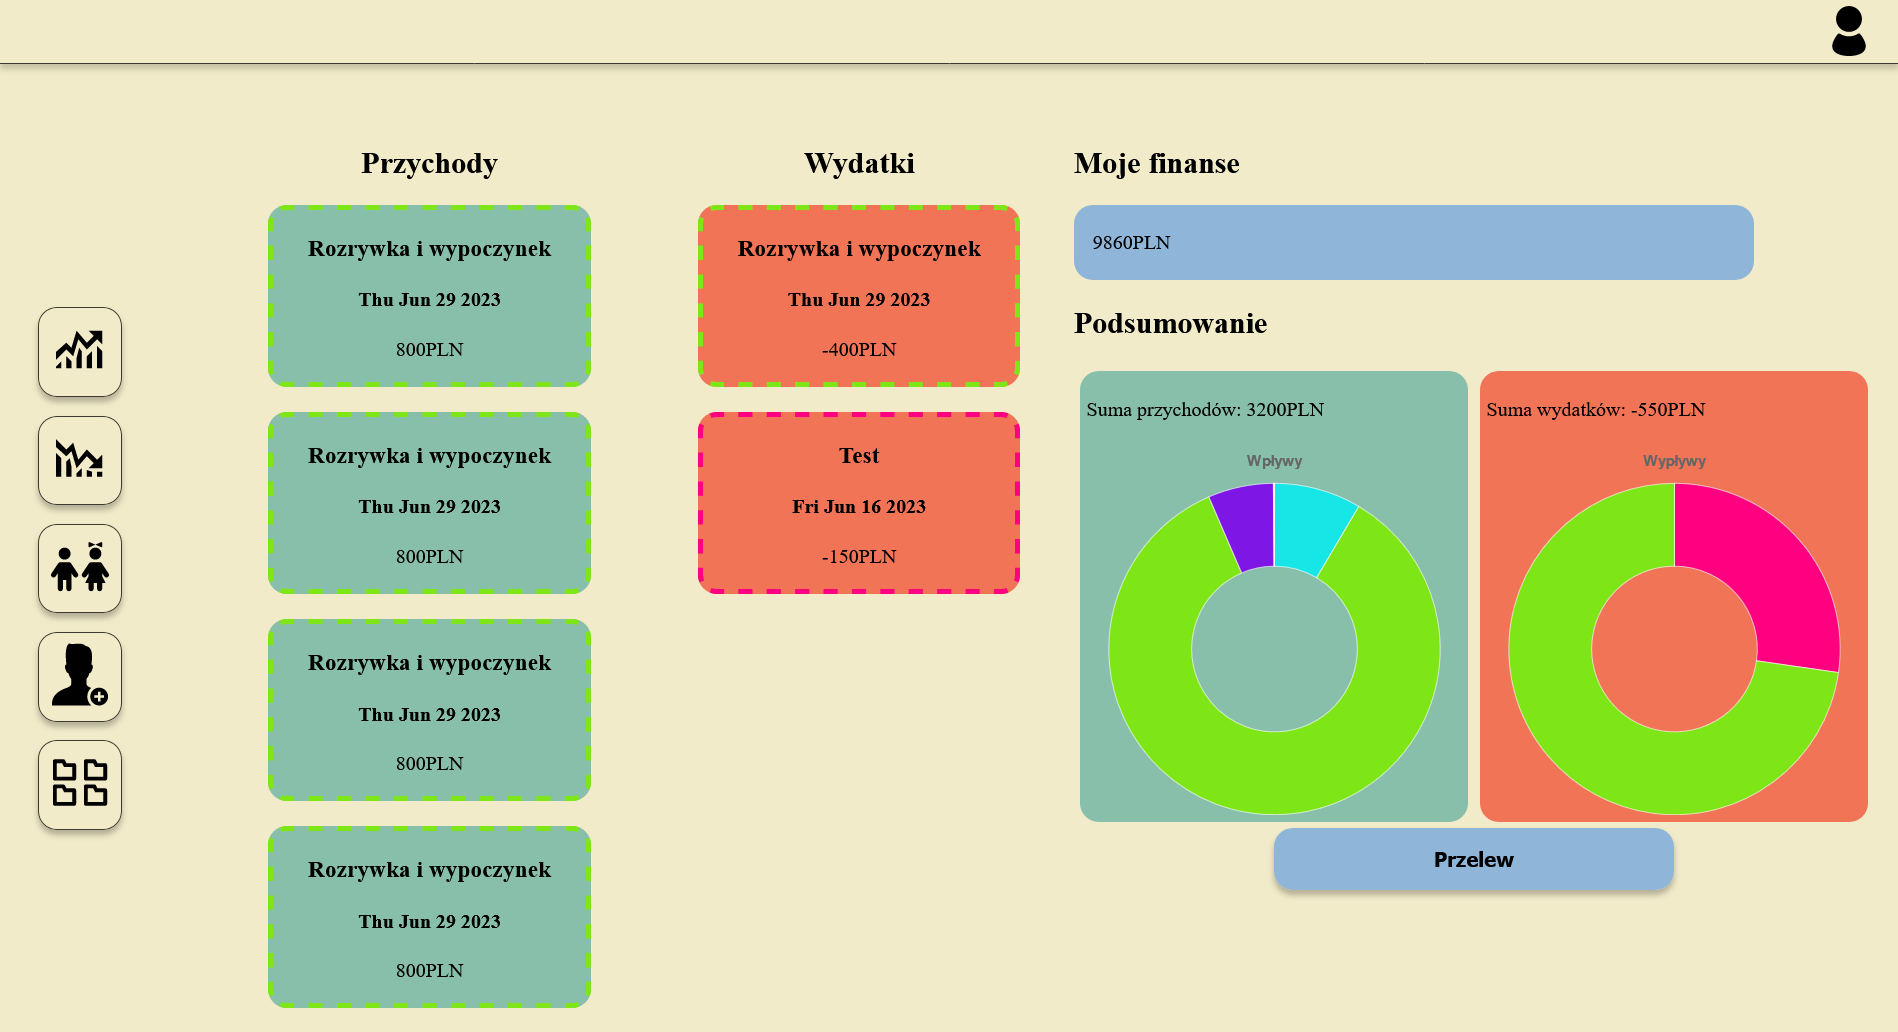
\includegraphics[width=\hsize,keepaspectratio]{images/profile.png}
    \caption{Zrzut ekranu głównego aplikacji.}
\end{figure}
Poprawne logowanie skutkuje przeniesieniem użytkownika do ekranu głównego
aplikacji. Zakładka \textbf{moje finanse} informuje korzystającego z systemu o
aktualnym stanie konta. Wyświetlana po lewej stronie lista \textbf{przychodów}
oraz \textbf{wydatków} wyświetla ostatnio dodane operacje. Lista ta zawiera 
cztery ostatnie dodane rekordy, wraz z nazwą kategorii, do jakiej operacja
została przypisana, datą wykonania oraz kwotą. Co więcej, ów lista zawiera
kolorową ramkę w kolorze przypisanym do danej kategorii, by pomóc korzystającemu
z aplikacji rozróżnić kategorie operacji. Sekcja \textbf{podsumowanie}
prezentuje zsumowane kwoty wydatków i przychodów, a pod wartościami wyświetlone
są wykresy kołowe operacji wykonanych w ostatnim miesiącu,
które prezentują podział operacji na kategorie i ich udział w
całkowitej sumie operacji. Poniżej podsumowania znajduje się przycisk
\textbf{Przelew}, który pozwala na przetransferowanie kwoty wewnątrz konta
pomiędzy profilami. Zostaną wtedy utworzone stosowne rekordy na profilu źródłowym
oraz docelowym. Ikony znajdujące się przy lewej krawędzi strony odpowiadają za
przejście do karty wydatków lub przychodów, dodanie konta dziecka, konta
z pełnymi uprawnieniami oraz kategorii.

\subsection{Profil dziecka}
\begin{figure}[H]
    \centering
    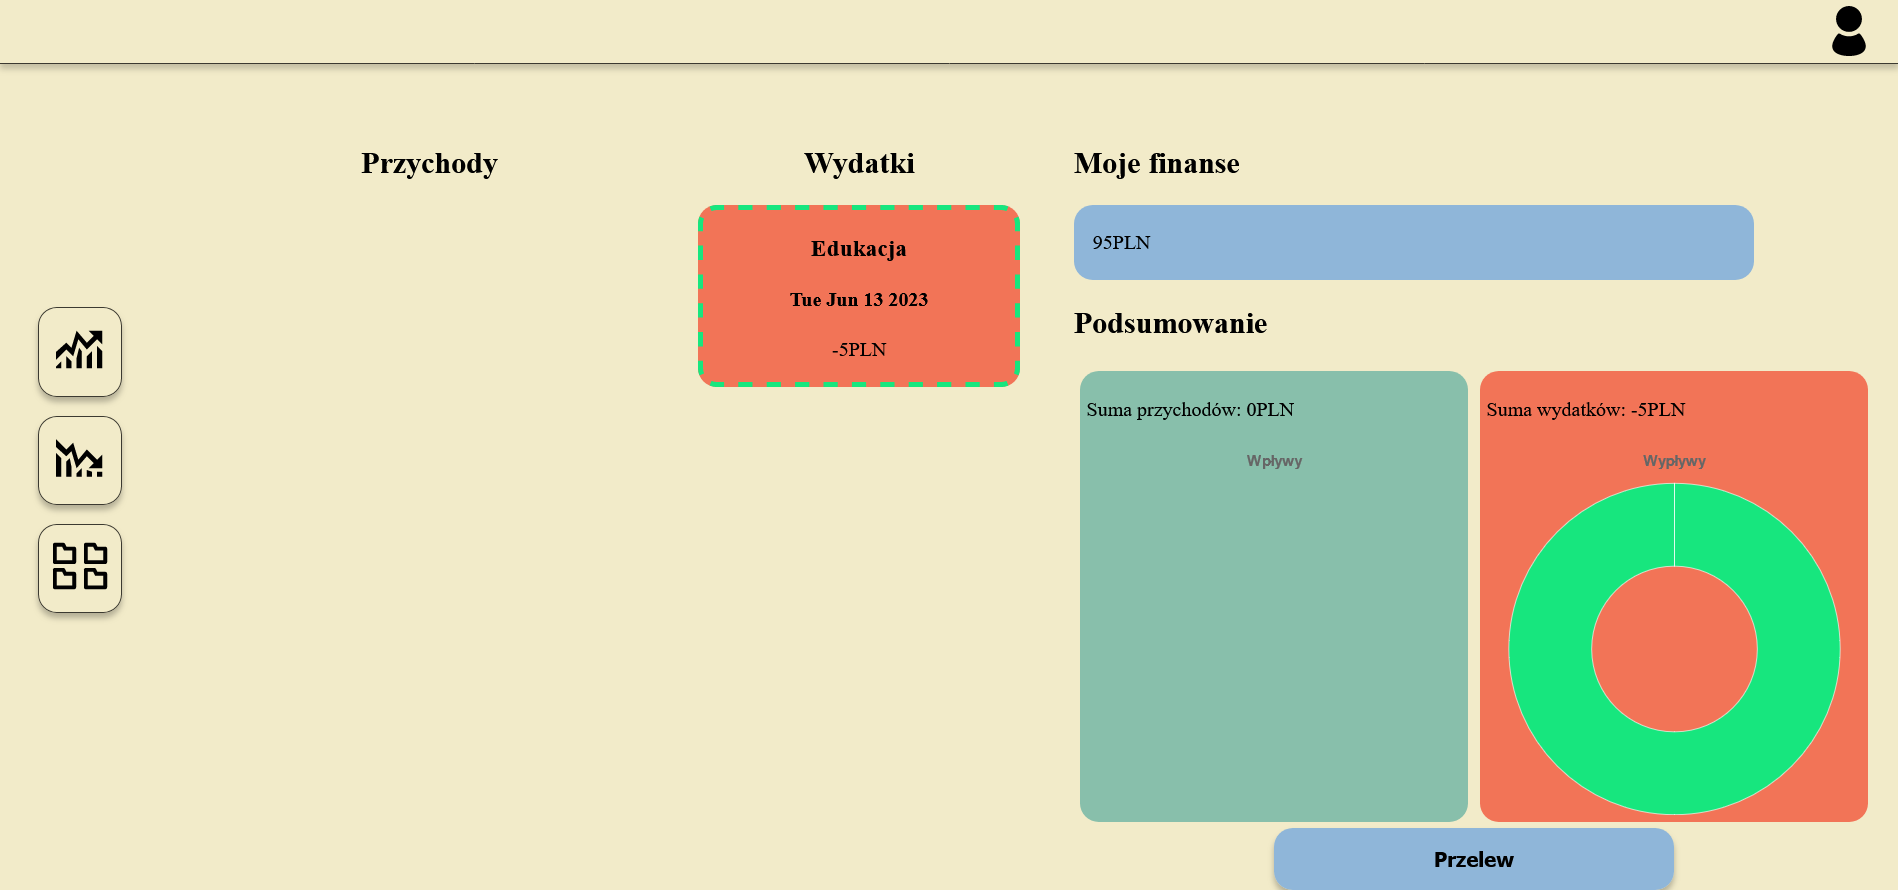
\includegraphics[width=\hsize,keepaspectratio]{images/childs_profile.png}
    \caption{Zrzut ekranu głównego dziecka.}
\end{figure}
Ekran główny dziecka zawiera mniej opcji niż panel dorosłego. Profil może
jedynie wykonać przelew wewnętrzny, wygenerować raport, wyświetlić kartę
wydatków oraz przychodów, dodawać je oraz utworzyć niestandardową kategorię.

\subsection{Przychody}
\begin{figure}[H]
    \centering
    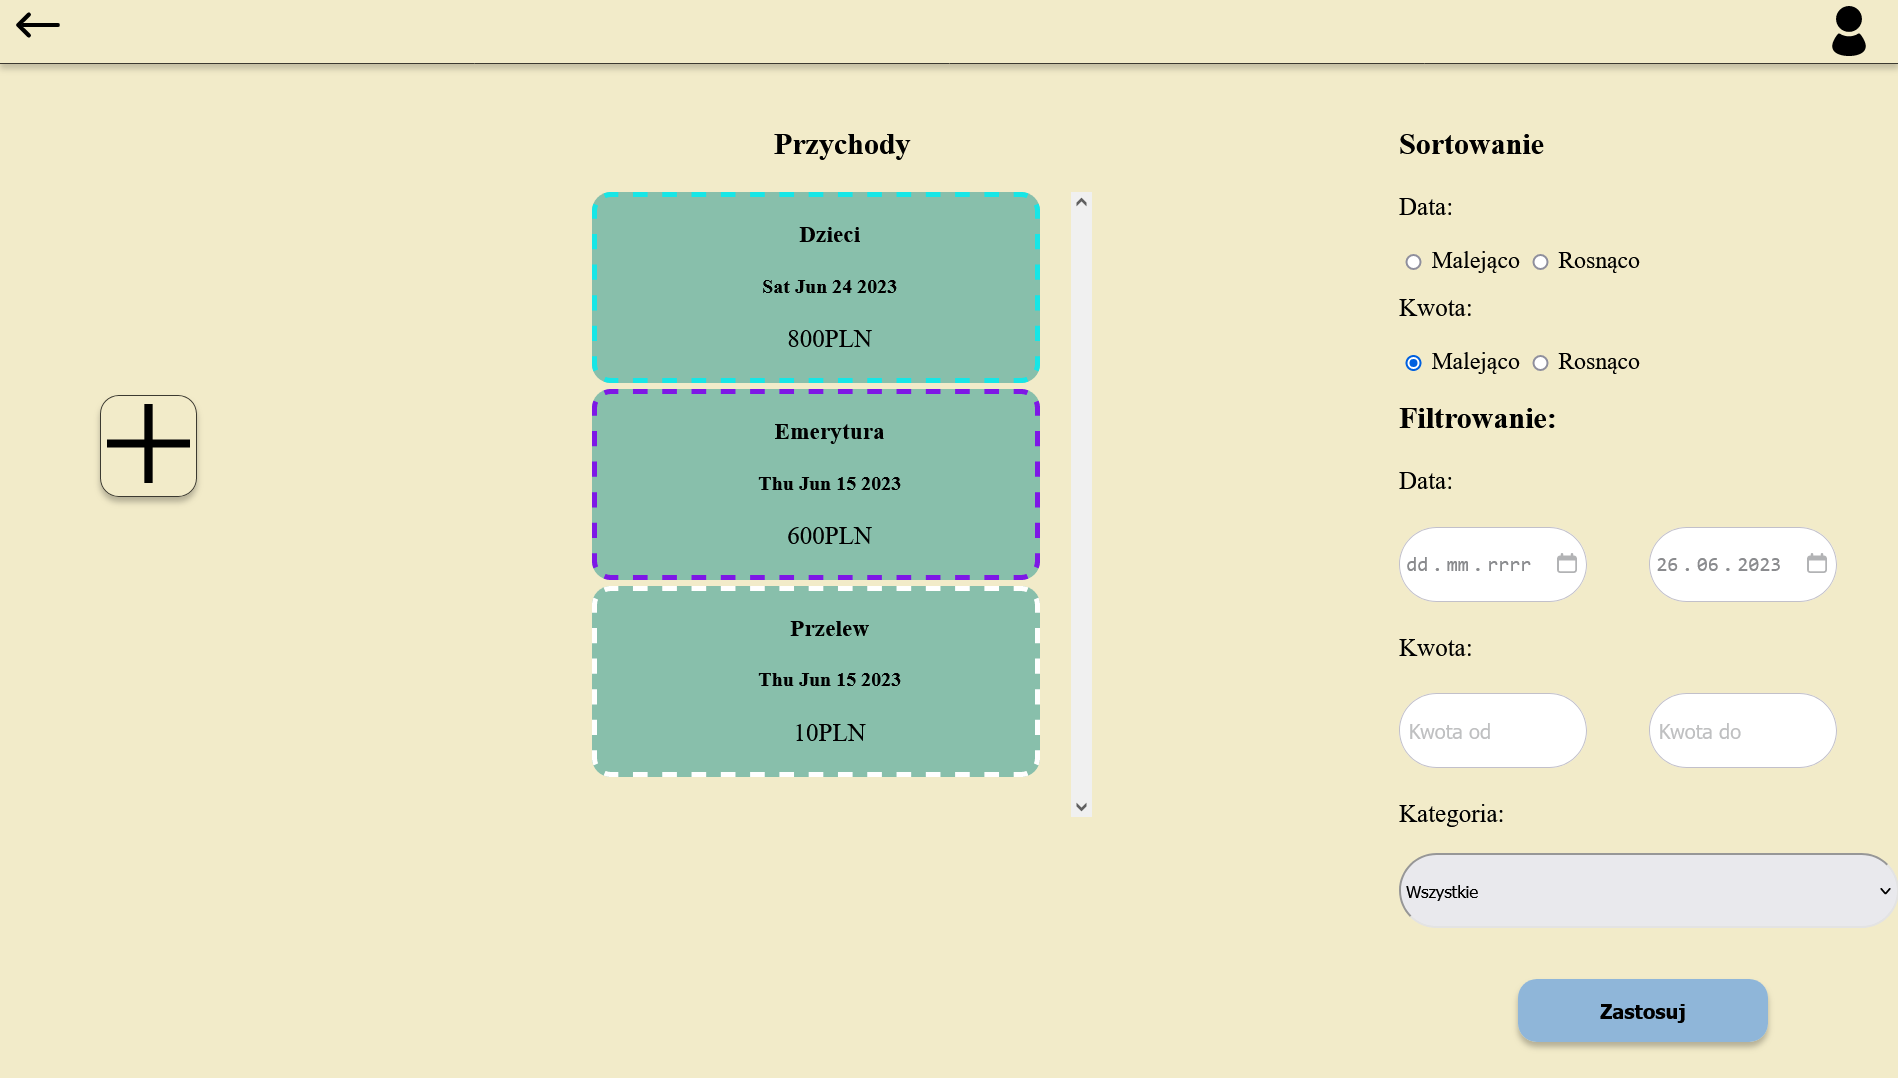
\includegraphics[width=\hsize,keepaspectratio]{images/incomes_card.png}
    \caption{Zrzut ekranu szczegółowego przychodów.}
\end{figure}
Po otworzeniu panelu \textbf{Przychody} użytkownikowi prezentowane są wszystkie
wykonane operacje, wraz z ich kwotą, datą wykonania oraz kategorią. Korzystający
z aplikacji ma możliwość sortowania oraz filtrowania względem daty, kwoty lub
kategorii za pomocą przycisku \textbf{Zastosuj}. Obok niego znajduje się 
przycisk \textbf{Generuj raport} pozwalający na wygenerowanie raportu z 
wykonanych operacji na koncie. Aby przejść do ekranu dodawania operacji, należy 
nacisnąć przycisk \textbf{+}.

\subsection{Wydatki}
\begin{figure}[H]
    \centering
    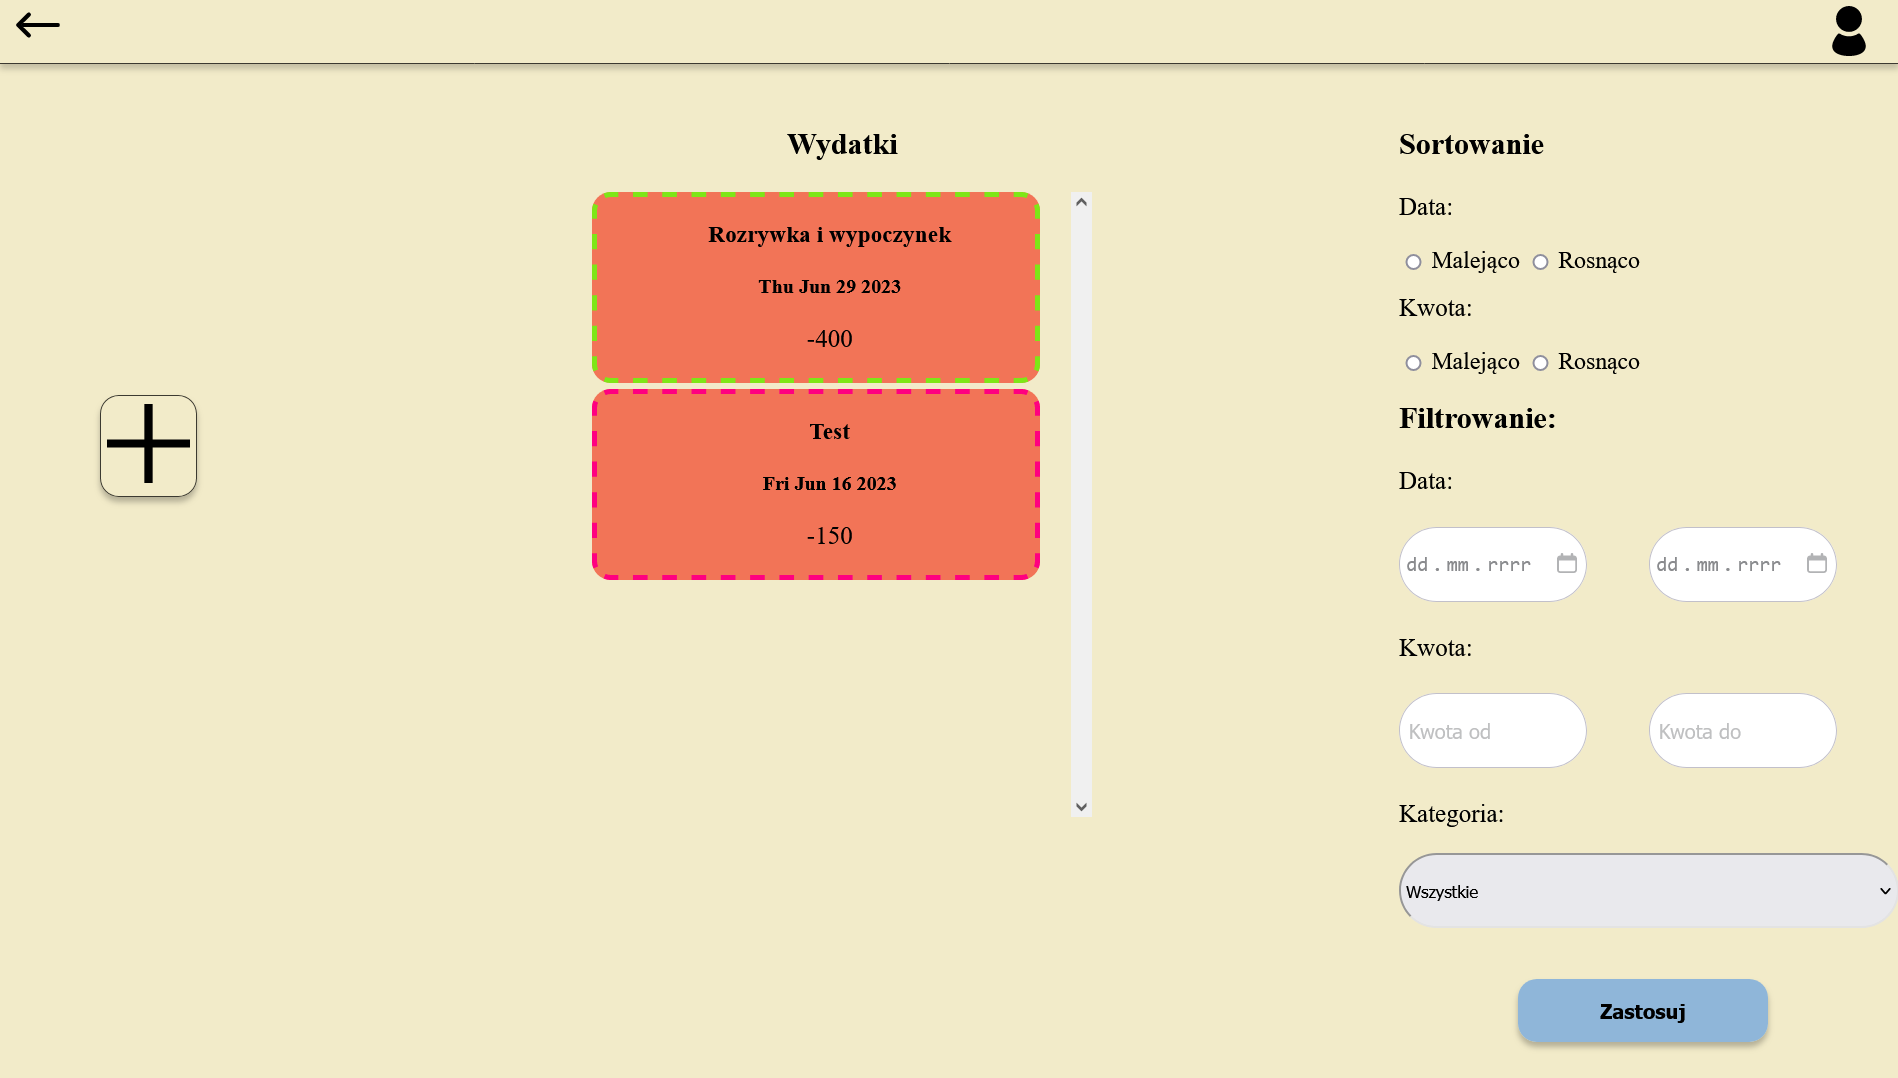
\includegraphics[width=\hsize,keepaspectratio]{images/expenses_card.png}
    \caption{Zrzut ekranu szczegółowego wydatków.}
\end{figure}
W przypadku wydatków ekran posiada analogiczne funkcje do ekranu dodawania
przychodów.

\subsection{Dodaj kategorię}
\begin{figure}[H]
    \centering
    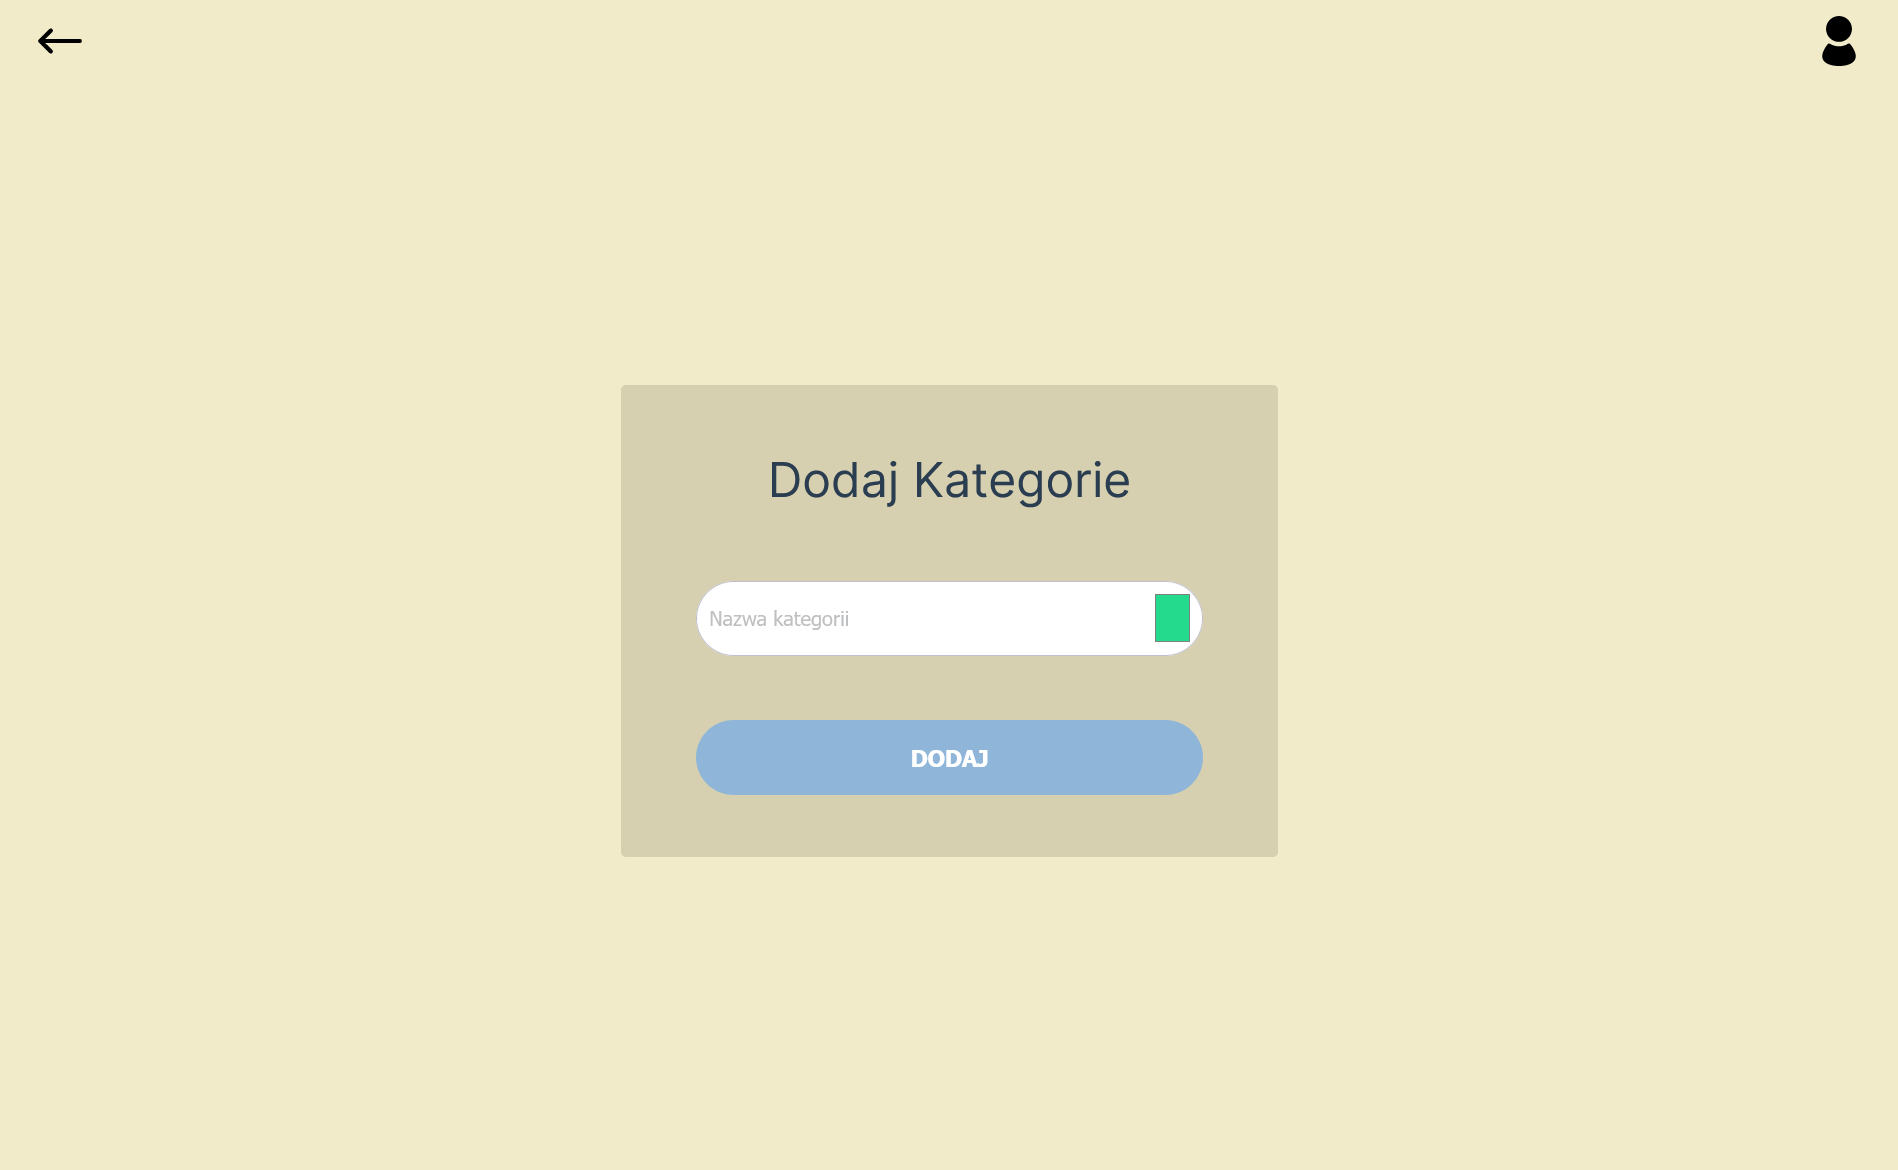
\includegraphics[width=\hsize,keepaspectratio]{images/add_category.png}
    \caption{Zrzut ekranu dodawania kategorii.}
\end{figure}
Ekran dodawania kategorii pozwala wprowadzić jej nazwę oraz nadać kolor.

\subsection{Dodawanie przychodów i wydatków}
\subsubsection{Dodaj przychód}
\begin{figure}[H]
    \centering
    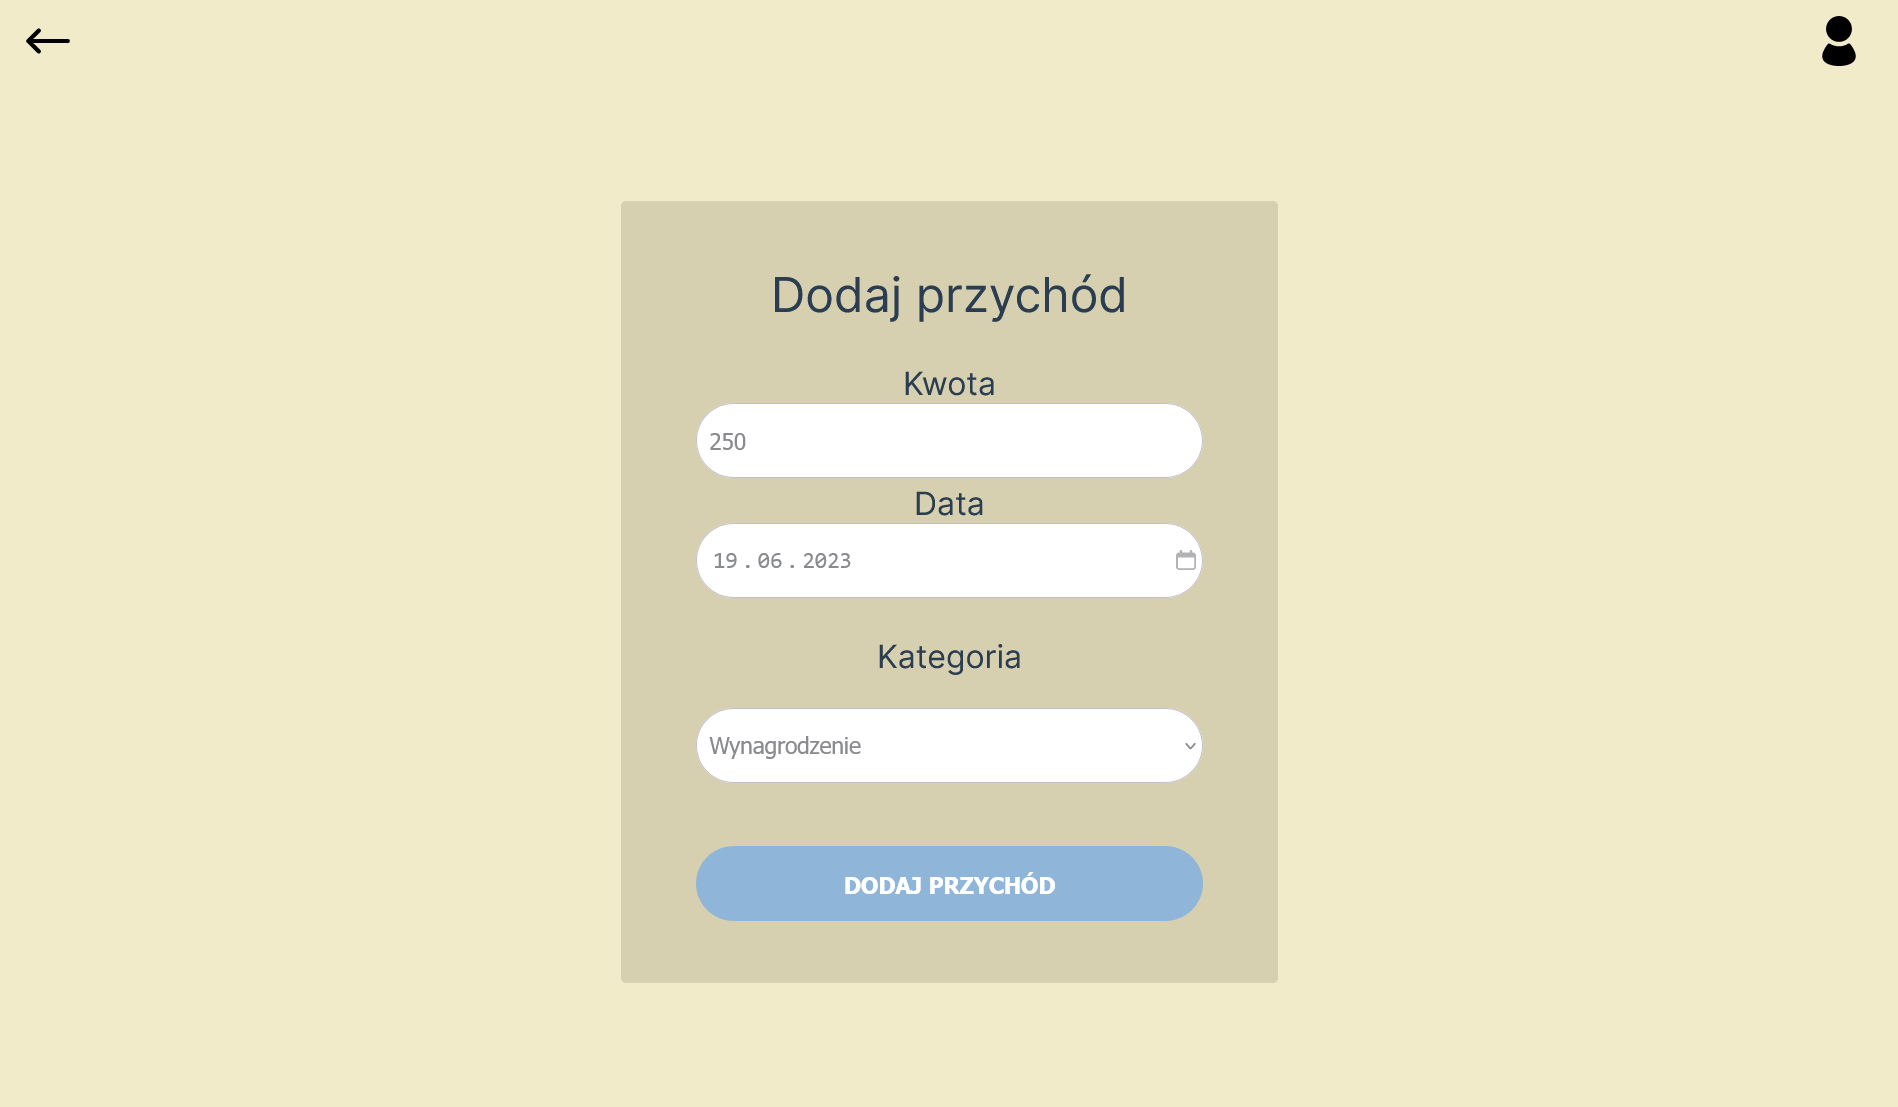
\includegraphics[width=\hsize,keepaspectratio]{images/add_income.png}
    \caption{Zrzut ekranu dodawania przychodu.}
\end{figure}
Ekran dodawania kategorii umożliwia wprowadzenie kwoty operacji, daty wykonania
oraz kategorii, do jakiej ów operacja należy.

\subsubsection{Dodaj wydatek}
\begin{figure}[H]
    \centering
    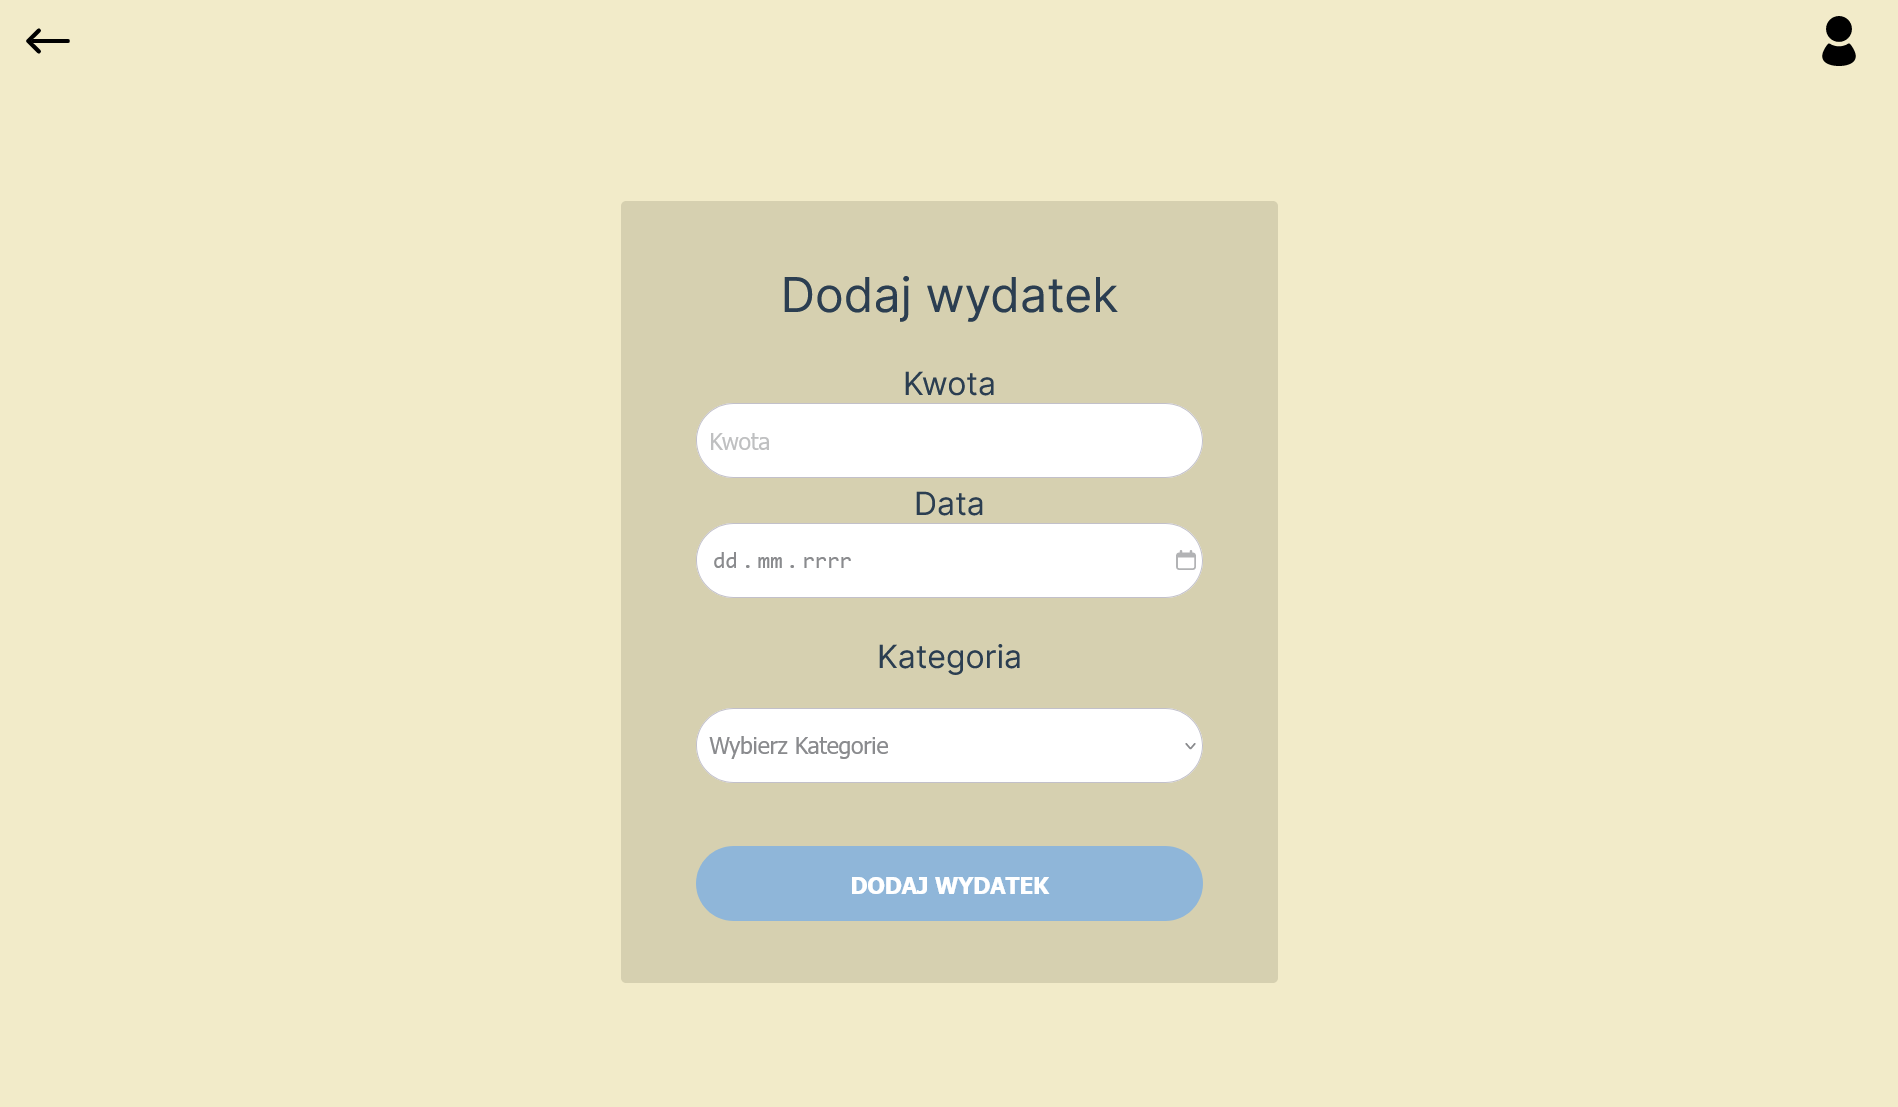
\includegraphics[width=\hsize,keepaspectratio]{images/add_expense.png}
    \caption{Zrzut ekranu dodawania wydatku.}
\end{figure}
W przypadku dodawania wydatku sytuacja jest analogiczna do dodawania przychodu.

\subsection{Wykonaj przelew}
\begin{figure}[H]
    \centering
    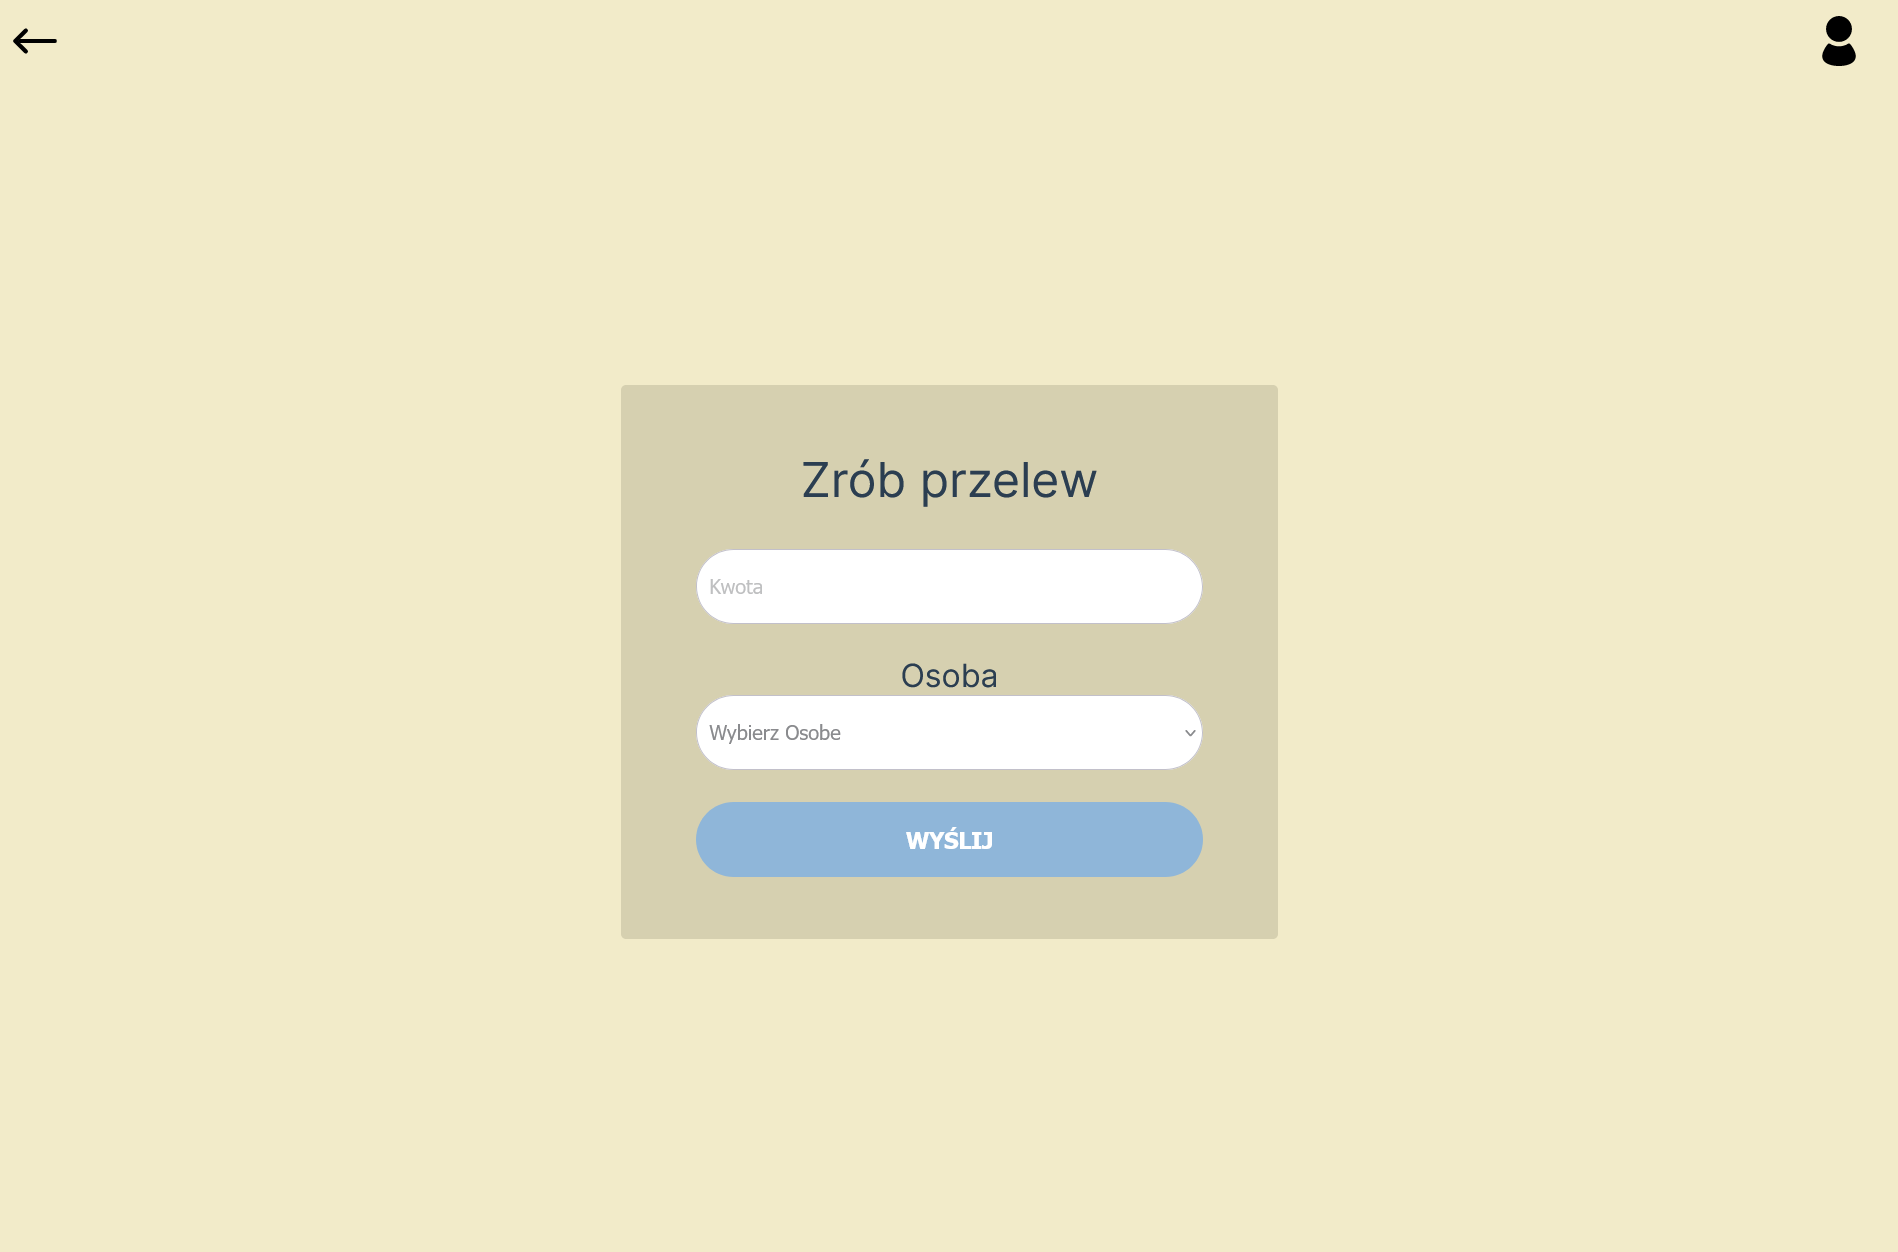
\includegraphics[width=\hsize,keepaspectratio]{images/make_transfer.png}
    \caption{Zrzut ekranu wykonywania przelewu.}
\end{figure}
Korzystający z aplikacji może wykonać przelew wewnętrzny pomiędzy kontami
należącymi do tej samej grupy. Aby to zrobić, należy podać kwotę oraz wybrać
profil docelowy.

\section{Specyfikacja wewnętrzna}
\subsection{Wykorzystane technologie}
System został wykonany w oparciu o technologię ASP.NET Web API. Wykorzystuje
Entity Framework do komunikacji z bazą danych SQL Server. Dokumentacja API
realizowana jest za pomocą frameworka Swagger.

% \subsection{Budowa systemu}

\subsection{Warstwy systemu}
\subsubsection{Warstwa bazy danych}
Warstwa ta jest odpowiedzialna za dostęp i modyfikację danych w bazie danych.
W niniejszej aplikacji użyto Entity Framework Core, który umożliwia korzystanie
z modelu obiektów i ułatwia wykonywanie operacji na danych.

\subsubsection{Warstwa logiki biznesowej}
Warstwa ta zaimplementowana jest w serwisach aplikacji i odpowiada za
przetwarzanie i filtrowanie danych zgodnie z założeniami biznesowymi aplikacji.
W kodzie przykładu ta warstwa jest reprezentowana przez klasy serwisów
\textbf{IAuthService}, \textbf{IAccountCreationService} i \textbf{IReportService}.

\subsubsection{Warstwa wizualna}
Warstwa wizualna odpowiada za prezentację danych w interfejsie użytkownika. 
W aplikacji jest reprezentowana przez generowanie punktów końcowych 
API zwracających kod HTML lub JSON i umożliwiających odwoływanie się do innych 
punktów końcowych. Warstwa wizualna korzysta z serwisów implementujących logikę 
biznesową.

\subsubsection{Warstwa autoryzacji}
Odpowiedzialna za zapewnienie mechanizmów uwierzytelniania i autoryzacji w 
systemie. W kodzie przykładu ta warstwa jest reprezentowana przez autoryzację 
ogólną JWT i autoryzację podziału dzielonych dla zasobów i tokenów 
uwierzytelniania.

% \subsection{Moduły systemu}

\section{Weryfikacja osiągniętych efektów względem założeń}
\subsection{Schemat zaimplementowanej bazy danych}
\begin{figure}[H]
    \centering
    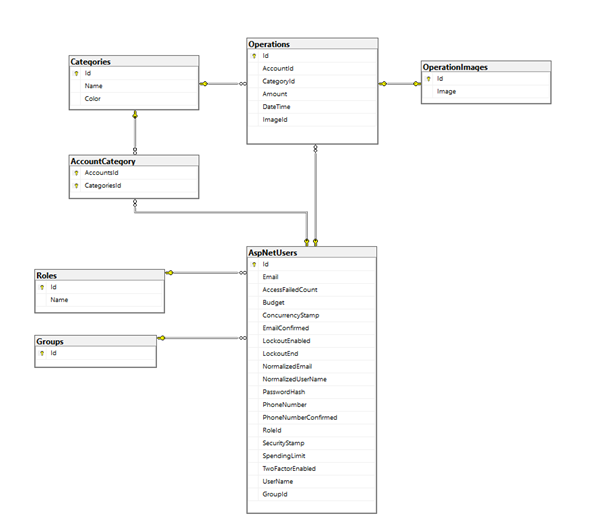
\includegraphics[width=\hsize,keepaspectratio]{images/DB2.png}
    \caption{Wykorzystany schemat bazy danych.}
\end{figure}

\subsection{Analiza wymagań i ich zmian względem założeń}
\subsubsection{Analiza wymagań funkcjonalnych}
Końcowa wersja aplikacji nie zawiera funkcjonalności przechowywania skanów
paragonów i faktur. Baza danych jest wyposażona w przechowywanie tych informacji,
jednak brakuje logiki w systemie. Brakuje jej również przechowywania informacji 
o dłużnikach. Funkcjonalność dodawania członków rodziny do konta jest rozwiązania 
w inny sposób, niż pierwotnie planowano. Konta łączone są w grupy, jednak każde
konto posiada osobne dane logowania. Początkowe założenie opierało się na jednym
koncie i zawierających się w nim profilach. Użycie osobnego hasła dla każdego
konta jest lepszym rozwiązaniem. Zaprezentowana przez nas aplikacja nie jest 
wyposażona w zarządzanie operacjami na koncie bankowym. Systemowi brakuje
dodanie cyklicznych/stałych operacji. W przypadku analizy MoSCoW i 
funkcjonalności Won't zawarto w aplikacji powiadomienia o przekroczonym budżecie 
dla konta dziecka, wynikające z jego typu i ograniczonego budżetu.

\subsubsection{Analiza wymagań niefunkcjonalnych}
W przypadku wymagań niefunkcjonalnych nie zostało zaimplementowane tworzenie
okresowych kopii zapasowych. System nie posiada również możliwości przypominania
hasła użytkownika. Potwierdzenie rejestracji e-mailem zostało wyłączone.

\section{Testowanie i uruchamianie}
System testowano w miarę budowania aplikacji oraz dodawania nowych
funkcjonalności. Ze względu na ograniczony czas realizacji projektu nie
wykonano testów jednostkowych na systemie. Pomimo tego aplikacja pracuje
poprawnie w ,,codziennym'' użytkowaniu. Nie zaobserwowano oczywistych problemów
podczas typowego korzystania. W miarę prac implementacyjnych pojawiały się błędy
typu semantycznego, które na bieżąco były rozwiązywane.

\section{Uwagi i wnioski}
Projekt realizowaliśmy w ciągu kilku miesięcy semestru akademickiego. W praktyce,
posiadając wiele innych obowiązków, stwierdzamy, że czas możliwy na realizację
projektu był zbyt krótki, by zapewnić pełną funkcjonalność aplikacji oraz wykonać
odpowiednie testy systemu. Niewątpliwie realizacja projektu pomogła nam w 
praktycznym zrozumieniu wykorzystanych przez nas technologii i stanowi cenne 
źródło wiedzy, którą najprawdopodobniej wykorzystamy podczas pracy w projektach
komercyjnych.

\end{document}
